% ============================================================
%  defense.tex
%  BTC Direction Prediction Using KANs Within the AFML Framework
%  Master's Final Work in Mathematical Finance  |  ISEG / ULisboa
%  Author: Petr Terletskiy
%  Supervisor: Prof. Joao Afonso Bastos
%
%  v3: Layout and content fixes per follow-up review.
% ============================================================

\documentclass[aspectratio=169, t]{beamer}

% ------------------------------------------------------------
%  Theme + ISEG colour palette
% ------------------------------------------------------------

\usetheme{Madrid}

\definecolor{isegred}{RGB}{166, 25, 46}

\setbeamercolor{structure}{fg=isegred}
\setbeamercolor{frametitle}{bg=isegred, fg=white}
\setbeamercolor{itemize item}{fg=isegred}
\setbeamercolor{itemize subitem}{fg=isegred!80}
\setbeamercolor{section in toc}{fg=isegred}
\setbeamercolor{subsection in toc}{fg=isegred!80}

\setbeamercolor{title}{fg=white}
\setbeamercolor{subtitle}{fg=white}
\setbeamercolor{author}{fg=black}
\setbeamercolor{institute}{fg=black}
\setbeamercolor{date}{fg=black}

\setbeamercolor{block title}{bg=gray!18, fg=black}
\setbeamercolor{block body}{bg=gray!5, fg=black}
\setbeamercolor{block title example}{bg=gray!18, fg=green!45!black}
\setbeamercolor{block body example}{bg=gray!5, fg=black}
\setbeamercolor{block title alerted}{bg=isegred!12, fg=isegred}
\setbeamercolor{block body alerted}{bg=isegred!4, fg=black}

\setbeamertemplate{navigation symbols}{}

% Palette for problems and contributions
\definecolor{probred1}{RGB}{139, 26, 26}
\definecolor{probred2}{RGB}{200, 80, 80}
\definecolor{contgreen1}{RGB}{30, 95, 50}
\definecolor{contgreen2}{RGB}{96, 165, 90}

% ------------------------------------------------------------
%  Packages
% ------------------------------------------------------------

\usepackage[utf8]{inputenc}
\usepackage[T1]{fontenc}
\usepackage[english]{babel}
\usepackage{lmodern}

\usepackage{amsmath, amssymb, amsthm, mathtools}
\usepackage{booktabs}
\usepackage{array}
\usepackage{multicol}

\usepackage{graphicx}
\graphicspath{{figures/}}

\usepackage{xcolor}
\usepackage{caption}
\captionsetup{font=small, labelfont={color=isegred, bf}}

\usepackage{tikz}
\usetikzlibrary{
  arrows.meta,
  positioning,
  shapes.geometric,
  calc,
  fit,
  backgrounds,
  decorations.pathmorphing,
  decorations.markings
}

\usepackage{hyperref}
\hypersetup{colorlinks=true, linkcolor=isegred, urlcolor=isegred}

% ------------------------------------------------------------
%  Math shortcuts
% ------------------------------------------------------------

\DeclareMathOperator*{\argmax}{argmax}
\DeclareMathOperator*{\argmin}{argmin}
\DeclareMathOperator{\sgn}{sgn}

\newcommand{\R}{\mathbb{R}}
\newcommand{\Prob}{\mathbb{P}}
\newcommand{\Ex}{\mathbb{E}}

% ------------------------------------------------------------
%  Param tracker for Phase I (top-right corner)
% ------------------------------------------------------------
\newcommand{\paramsbox}[4]{%
  \begin{tikzpicture}[remember picture, overlay]
    \node[anchor=north east, xshift=-0.3cm, yshift=-0.1cm]
      at (current page.north east) {%
      \begin{tikzpicture}[
        param/.style={
          draw, rounded corners=2pt, line width=0.5pt,
          minimum width=8mm, minimum height=6.5mm,
          font=\footnotesize\bfseries, inner sep=1pt
        },
        lit/.style={fill=green!35, draw=green!50!black, text=green!40!black},
        act/.style={fill=yellow!45, draw=orange!85, text=orange!55!black},
        dim/.style={fill=gray!20, draw=gray!50, text=gray!60!black}
      ]
        \node[param, #1] (Xn) at (0,    0) {$X$};
        \node[param, #2] (Yn) at (0.9,  0) {$y$};
        \node[param, #3] (Wn) at (1.8,  0) {$w$};
        \node[param, #4] (Tn) at (2.7,  0) {$t_1$};
      \end{tikzpicture}
    };
  \end{tikzpicture}%
}

% ------------------------------------------------------------
%  Title page metadata
% ------------------------------------------------------------

\title[BTC Direction with KANs]
      {Bitcoin Price Direction Prediction Using Kolmogorov-Arnold Networks\\Within the Advances in Financial Machine Learning Framework}

\subtitle{Master's Final Work in Mathematical Finance}

\author[P. Terletskiy]{Petr Terletskiy}

\institute[ISEG / ULisboa]{%
  ISEG, Lisbon School of Economics \& Management \\
  Universidade de Lisboa \\[0.4em]
  \small Supervisor: Prof.\ Jo\~ao Afonso Bastos
}

\date{22 July 2026}

\titlegraphic{\vspace{0.3cm}\includegraphics[height=1.2cm]{ISEG_logo.png}}

\begin{document}

% =========================================================
%  COVER
% =========================================================
\begin{frame}[plain]
  \titlepage
\end{frame}

% =========================================================
%  TABLE OF CONTENTS  
% =========================================================
\begin{frame}{Table of contents}
\vspace{0.8em}

\begin{minipage}[t][0.72\textheight][t]{\linewidth}

  \textbf{\color{isegred}\large 1. Problems and Contributions}

  \vfill

  \textbf{\color{isegred}\large 2. KAN theoretical background}
  \begin{itemize}\footnotesize
    \item From representation theorem to neural network.
  \end{itemize}

  \vfill

  \textbf{\color{isegred}\large 3. Methodology}
  \begin{itemize}\footnotesize
    \item Phase I $\rightarrow$ Phase II $\rightarrow$ Phase III.
  \end{itemize}

  \vfill

  \textbf{\color{isegred}\large 4. Results}
  \begin{itemize}\footnotesize
    \item Two questions, two answers.
  \end{itemize}

  \vfill

  \textbf{\color{isegred}\large 5. Limitations and future work}

  \vfill

  \textbf{\color{isegred}\large 6. Conclusion}

\end{minipage}
\end{frame}

% =========================================================
%  HOOK  -  Origin story: the question that started the thesis
% =========================================================
\begin{frame}[c]{Where this started}

\centering

{\large This thesis began with one question:}

\vspace{0.6em}


\begin{tikzpicture}
\node[draw=isegred, fill=isegred!6, rounded corners=5pt, line width=1.2pt,
      text width=10cm, align=center, inner sep=11pt]
  {\Large\itshape Does on-chain data help predict\\[0.15em] Bitcoin's price direction?};
\end{tikzpicture}

\vspace{1.0em}

{\large To answer it, I turned to the literature and found}

\vspace{0.4em}

{\fontsize{34}{40}\selectfont\bfseries\color{isegred} 80--90\% accuracy}

\vspace{0.4em}

{\large reported everywhere, on pipelines that leak the future.}

\vspace{0.8em}

{\footnotesize\itshape Before I could trust any answer to my question, the evaluation had to be rebuilt.}

\vspace{0.5em}

{\scriptsize That rebuild follows the \textbf{AFML} framework of López de Prado (2018).}

\end{frame}

% =========================================================
%  HOOK 2  -  Why KAN: a network you can read
% =========================================================
\begin{frame}[c]{A different kind of model}

\centering

{\large Most neural networks are black boxes.}

\vspace{0.5em}

{\normalsize You get a prediction, never a reason.}

\vspace{1.4em}

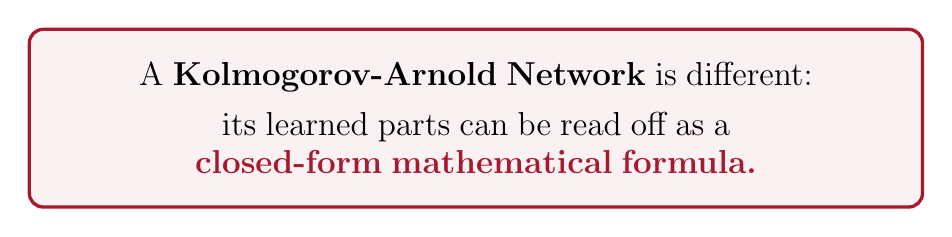
\begin{tikzpicture}
\node[draw=isegred, fill=isegred!6, rounded corners=5pt, line width=1.2pt,
      text width=10.5cm, align=center, inner sep=12pt]
  {\large A \textbf{Kolmogorov-Arnold Network} is different:\\[0.35em]
   its learned parts can be read off as a\\[0.15em]
   \textbf{\color{isegred} closed-form mathematical formula.}};
\end{tikzpicture}

\vspace{1.4em}

{\large So it offers something the others cannot: \textbf{\color{isegred}interpretability.}}

\vspace{1.0em}

{\footnotesize\itshape And that transparency does not depend on the prediction being good.}

\end{frame}

% =========================================================
%  Contributions (single slide)
% =========================================================
\begin{frame}[c]{Contributions}
\centering

{\footnotesize Two threads, four contributions.}

\vspace{1.2em}

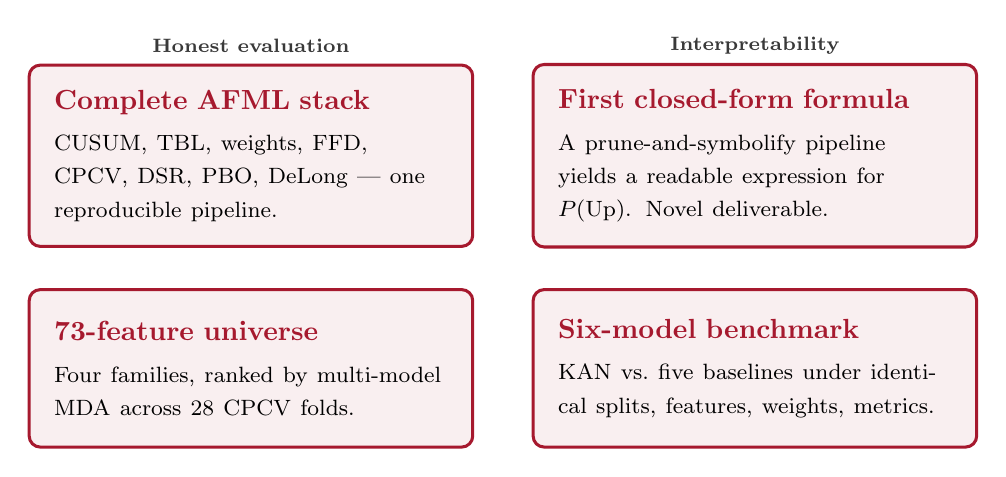
\begin{tikzpicture}[
    cbox/.style={
        draw=isegred, fill=isegred!7, rounded corners=4pt, line width=1.1pt,
        text width=5.0cm, minimum height=2.0cm,
        align=left, inner sep=9pt
    },
  thlbl/.style={font=\scriptsize\bfseries, text=gray!45!black}
]
\def\rA{1.35}   \def\rB{-1.35}
\def\xL{-3.2}   \def\xR{3.2}

\node[thlbl] at (\xL, 2.75) {Honest evaluation};
\node[thlbl] at (\xR, 2.75) {Interpretability};

\node[cbox] at (\xL,\rA) {%
  {\bfseries\color{isegred}Complete AFML stack}\\[3pt]
  {\footnotesize CUSUM, TBL, weights, FFD, CPCV, DSR, PBO, DeLong \textemdash\ one reproducible pipeline.}
};

\node[cbox] at (\xR,\rA) {%
  {\bfseries\color{isegred}First closed-form formula}\\[3pt]
  {\footnotesize A prune-and-symbolify pipeline yields a readable expression for $P(\mathrm{Up})$. Novel deliverable.}
};

\node[cbox] at (\xL,\rB) {%
  {\bfseries\color{isegred}73-feature universe}\\[3pt]
  {\footnotesize Four families, ranked by multi-model MDA across 28 CPCV folds.}
};

\node[cbox] at (\xR,\rB) {%
  {\bfseries\color{isegred}Six-model benchmark}\\[3pt]
  {\footnotesize KAN vs.\ five baselines under identical splits, features, weights, metrics.}
};

\end{tikzpicture}
\end{frame}

% =========================================================
%  KAN representation theorem
% =========================================================
\begin{frame}{Kolmogorov-Arnold representation theorem}

\vspace{-0.6em}

{
\setbeamercolor{block title}{bg=isegred!12, fg=isegred}
\setbeamercolor{block body}{bg=isegred!3, fg=black}
\begin{block}{Theorem}
\centering
Any continuous function $f : [0,1]^n \to \mathbb{R}$ decomposes \\
as a finite sum of continuous univariate functions:

\vspace{0.6em}

{\large
$\displaystyle f(x_1, \ldots, x_n) \;=\; \sum_{q=1}^{2n+1} \Phi_q\!\left( \sum_{p=1}^{n} \phi_{q,p}(x_p) \right)$
}
\end{block}
}

\vspace{0.5em}

\begin{itemize}
  \item $\phi_{q,p}$ and $\Phi_q$ are continuous univariate functions.
  \item Addition is the only genuinely multivariate operation.
  \item Long considered useless for neural networks (the inner $\phi_{q,p}$ can be highly non-smooth), until Liu et al.\ (2024).
\end{itemize}

\vfill
\hfill {\scriptsize\itshape\color{gray} Kolmogorov (1957), Arnold (1958)}

\end{frame}


% =========================================================
%  From theorem to network
% =========================================================
\begin{frame}{From theorem to network}

\vspace{-0.4em}
\begin{center}
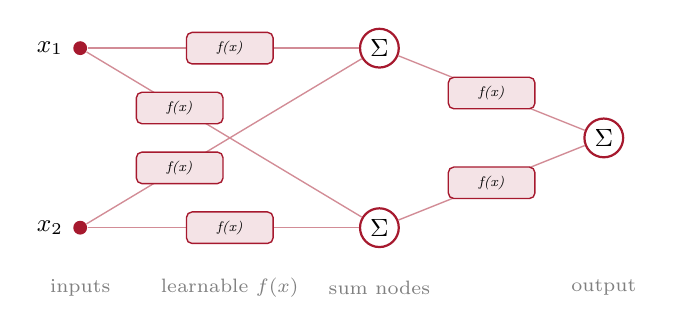
\begin{tikzpicture}[
  scale=0.95,
  xnode/.style={circle, fill=isegred, minimum size=5pt, inner sep=0pt},
  snode/.style={circle, draw=isegred, fill=white, line width=0.8pt,
                minimum size=14pt, inner sep=0pt, font=\small},
  fxbox/.style={
    draw=isegred, rounded corners=2pt, line width=0.5pt,
    fill=isegred!12, font=\tiny\itshape,
    inner sep=2pt, minimum width=11mm, minimum height=4mm
  },
  edge/.style={draw=isegred!50, line width=0.5pt}
]

\node[xnode, label=left:{\small$x_1$}] (x1) at (0, 1.2) {};
\node[xnode, label=left:{\small$x_2$}] (x2) at (0, -1.2) {};

\node[snode] (h1) at (4, 1.2)  {$\Sigma$};
\node[snode] (h2) at (4, -1.2) {$\Sigma$};

\node[snode] (y) at (7, 0) {$\Sigma$};

\draw[edge] (x1) -- (h1);  \draw[edge] (x1) -- (h2);
\draw[edge] (x2) -- (h1);  \draw[edge] (x2) -- (h2);
\draw[edge] (h1) -- (y);   \draw[edge] (h2) -- (y);

\node[fxbox] at (2.0,  1.2)  {f(x)};
\node[fxbox] at (2.0, -1.2)  {f(x)};
\node[fxbox] at (1.33,  0.4) {f(x)};
\node[fxbox] at (1.33, -0.4) {f(x)};
\node[fxbox] at (5.5,  0.6)  {f(x)};
\node[fxbox] at (5.5, -0.6)  {f(x)};

\node[font=\scriptsize, color=gray] at (0, -2.0) {inputs};
\node[font=\scriptsize, color=gray] at (2, -2.0) {learnable $f(x)$};
\node[font=\scriptsize, color=gray] at (4, -2.0) {sum nodes};
\node[font=\scriptsize, color=gray] at (7, -2.0) {output};

\end{tikzpicture}
\end{center}

\vspace{0.3em}

\begin{itemize}
  \item \textbf{A learnable univariate function on every edge}, parameterised as a B-spline.
  \item \textbf{Fewer parameters than an MLP.} The B-spline economy matters for the 1{,}168-event sample.
  \item \textbf{Symbolifiable by construction.} Each 1D edge curve maps to a closed-form primitive (sin, cos, tanh, polynomial), giving interpretability that conventional deep architectures cannot.
\end{itemize}

\end{frame}

% =========================================================
%  PIPELINE OVERVIEW
% =========================================================
\begin{frame}[c]{Pipeline overview}

\centering

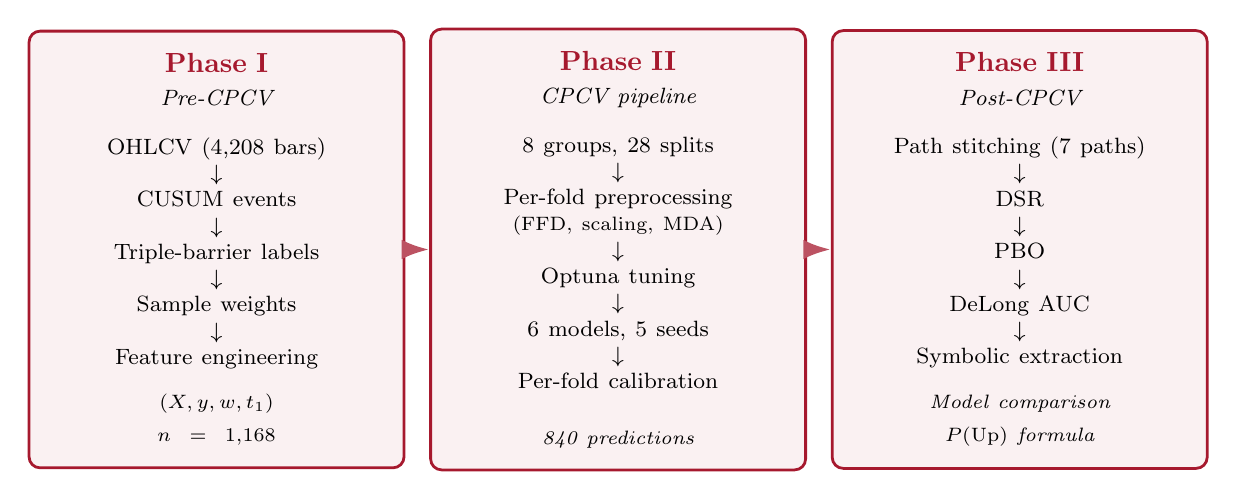
\begin{tikzpicture}[
  phasebox/.style={
    draw, rounded corners=4pt, line width=1pt,
    fill=isegred!6, draw=isegred,
    text width=4.2cm, minimum height=5.5cm,
    align=center, inner sep=8pt
  },
  arrow/.style={
    -{Latex[length=3.5mm, width=2.5mm]},
    line width=1.4pt, draw=isegred!75
  }
]

\node[phasebox] (p1) at (-5.1, 0) {%
  {\bfseries\color{isegred} Phase I}\\
  {\footnotesize\itshape Pre-CPCV}\\[8pt]
  \footnotesize
  OHLCV (4{,}208 bars)\\
  $\downarrow$\\
  CUSUM events\\
  $\downarrow$\\
  Triple-barrier labels\\
  $\downarrow$\\
  Sample weights\\
  $\downarrow$\\
  Feature engineering\\[8pt]
  {\scriptsize\itshape $(X, y, w, t_1)$\\$n = 1{,}168$}
};

\node[phasebox] (p2) at (0, 0) {%
  {\bfseries\color{isegred} Phase II}\\
  {\footnotesize\itshape CPCV pipeline}\\[8pt]
  \footnotesize
  8 groups, 28 splits\\
  $\downarrow$\\
  Per-fold preprocessing\\
  {\scriptsize (FFD, scaling, MDA)}\\
  $\downarrow$\\
  Optuna tuning\\
  $\downarrow$\\
  6 models, 5 seeds\\
  $\downarrow$\\
  Per-fold calibration\\[8pt]
  {\scriptsize\itshape 840 predictions}
};

\node[phasebox] (p3) at (5.1, 0) {%
  {\bfseries\color{isegred} Phase III}\\
  {\footnotesize\itshape Post-CPCV}\\[8pt]
  \footnotesize
  Path stitching (7 paths)\\
  $\downarrow$\\
  DSR\\
  $\downarrow$\\
  PBO\\
  $\downarrow$\\
  DeLong AUC\\
  $\downarrow$\\
  Symbolic extraction\\[8pt]
  {\scriptsize\itshape Model comparison\\$P(\mathrm{Up})$ formula}
};

\draw[arrow] (p1.east) -- (p2.west);
\draw[arrow] (p2.east) -- (p3.west);

\end{tikzpicture}

\end{frame}

% =========================================================
%  PHASE I  - Intro divider
% =========================================================
\begin{frame}[c]{Phase I: Pre-CPCV}

\centering
{\fontsize{56}{68}\selectfont\bfseries\color{isegred} Phase I}\\[0.4em]
{\Large\itshape Pre-CPCV}\\[1em]
{\normalsize From raw OHLCV to the aligned tuple $(X, y, w, t_1)$.}

\vspace{1.5em}


\begin{tikzpicture}[
  param/.style={
    draw, rounded corners=3pt, line width=1pt,
    minimum width=1.8cm, minimum height=1.4cm,
    font=\LARGE, inner sep=4pt,
    fill=gray!8, draw=gray!40, text=gray!55
  }
]
  \node[param] at (-3.6, 0) {$X$};
  \node[param] at (-1.2, 0) {$y$};
  \node[param] at ( 1.2, 0) {$w$};
  \node[param] at ( 3.6, 0) {$t_1$};
\end{tikzpicture}

\end{frame}

% =========================================================
%  PHASE I  - CUSUM event filter (EWMA provenance at top)
% =========================================================
\begin{frame}{Phase I: CUSUM event filter}
\paramsbox{dim}{dim}{dim}{dim}
\vspace{-3.7em}

\hspace*{-0.03\textwidth}%
\begin{columns}[T]
\begin{column}{0.31\textwidth}
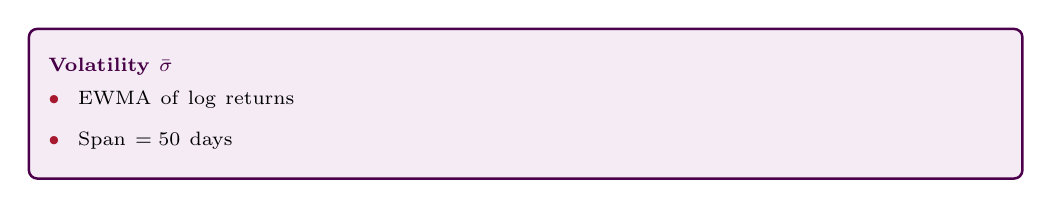
\begin{tikzpicture}
\node[draw=violet!60!black, fill=violet!8, rounded corners=3pt, line width=0.9pt,
      text width=\linewidth, align=left, inner sep=7pt, minimum height=1.9cm] {%
  \scriptsize\textbf{\color{violet!55!black}Volatility $\bar{\sigma}$}\\[4pt]
  \scriptsize \textcolor{isegred}{$\bullet$}~ EWMA of log returns\\[3pt]
  \scriptsize \textcolor{isegred}{$\bullet$}~ Span $= 50$ days};
\end{tikzpicture}
\end{column}
\begin{column}{0.02\textwidth}\hfill\end{column}
\begin{column}{0.68\textwidth}
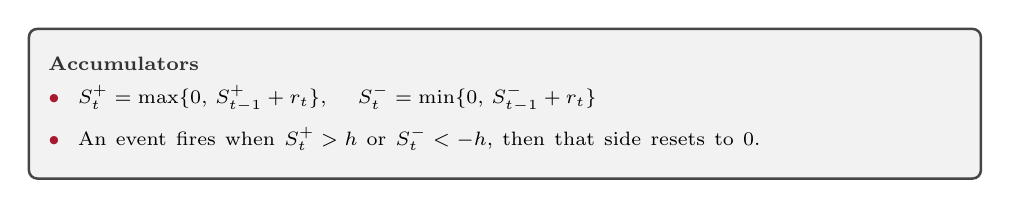
\begin{tikzpicture}
\node[draw=gray!55!black, fill=gray!10, rounded corners=3pt, line width=0.9pt,
      text width=\dimexpr\linewidth-15pt\relax, align=left, inner sep=7pt, minimum height=1.9cm] {%
  \scriptsize\textbf{\color{gray!40!black}Accumulators}\\[4pt]
  \scriptsize \textcolor{isegred}{$\bullet$}~ $S_t^+ = \max\{0,\, S_{t-1}^+ + r_t\}$, \quad $S_t^- = \min\{0,\, S_{t-1}^- + r_t\}$\\[3pt]
  \scriptsize \textcolor{isegred}{$\bullet$}~ An event fires when $S_t^+ > h$ or $S_t^- < -h$, then that side resets to 0.};
\end{tikzpicture}
\end{column}
\end{columns}

\vspace{0.5em}

\begin{center}
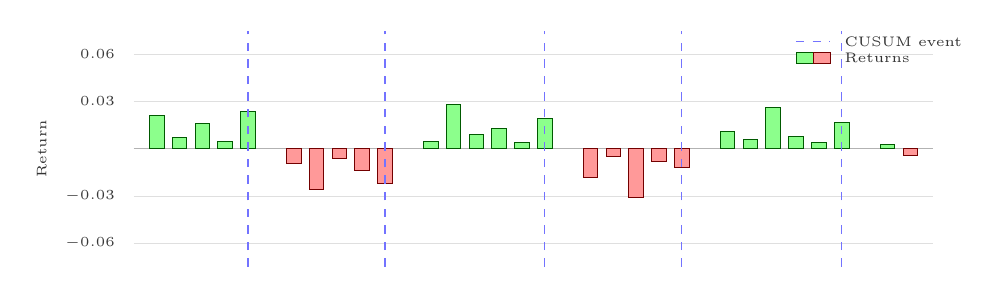
\begin{tikzpicture}[
  font=\tiny,
  xscale=0.29, yscale=20,
  posbar/.style={fill=green!45!white, draw=green!35!black, line width=0.2pt},
  negbar/.style={fill=red!40!white, draw=red!45!black, line width=0.2pt},
  evline/.style={draw=blue!55, dashed, line width=0.5pt}
]

% axis
\draw[draw=gray!60, line width=0.4pt] (0,0) -- (35,0);
\foreach \y in {-0.06,-0.03,0.03,0.06}{
  \draw[draw=gray!25, line width=0.2pt] (0,\y) -- (35,\y);
  \node[anchor=east, font=\tiny, text=gray!45!black] at (-0.4,\y) {$\y$};
}
\node[rotate=90, anchor=south, font=\tiny, text=gray!40!black] at (-3.4,0) {Return};

% --- run 1: positive accumulation, threshold reached at t=5 ---
\foreach \x/\v in {1/0.021, 2/0.007, 3/0.016, 4/0.005, 5/0.024}{
  \fill[posbar] (\x-0.32,0) rectangle (\x+0.32,\v);
}
\draw[evline] (5,-0.075) -- (5,0.075);

% --- run 2: negative accumulation, threshold reached at t=11 ---
\foreach \x/\v in {7/-0.009, 8/-0.026, 9/-0.006, 10/-0.014, 11/-0.022}{
  \fill[negbar] (\x-0.32,\v) rectangle (\x+0.32,0);
}
\draw[evline] (11,-0.075) -- (11,0.075);

% --- run 3: positive accumulation, threshold reached at t=18 ---
\foreach \x/\v in {13/0.005, 14/0.028, 15/0.009, 16/0.013, 17/0.004, 18/0.019}{
  \fill[posbar] (\x-0.32,0) rectangle (\x+0.32,\v);
}
\draw[evline] (18,-0.075) -- (18,0.075);

% --- run 4: negative accumulation, threshold reached at t=24 ---
\foreach \x/\v in {20/-0.018, 21/-0.005, 22/-0.031, 23/-0.008, 24/-0.012}{
  \fill[negbar] (\x-0.32,\v) rectangle (\x+0.32,0);
}
\draw[evline] (24,-0.075) -- (24,0.075);

% --- run 5: positive accumulation, threshold reached at t=31 ---
\foreach \x/\v in {26/0.011, 27/0.006, 28/0.026, 29/0.008, 30/0.004, 31/0.017}{
  \fill[posbar] (\x-0.32,0) rectangle (\x+0.32,\v);
}
\draw[evline] (31,-0.075) -- (31,0.075);

% --- tail: small mixed returns, no firing ---
\fill[posbar] (32.68,0) rectangle (33.32,0.003);
\fill[negbar] (33.68,-0.004) rectangle (34.32,0);

% legend
\draw[evline] (29.0,0.068) -- (30.5,0.068);
\node[anchor=west, font=\tiny, text=gray!40!black] at (30.7,0.068) {CUSUM event};
\fill[posbar] (29.0,0.054) rectangle (29.75,0.061);
\fill[negbar] (29.75,0.054) rectangle (30.5,0.061);
\node[anchor=west, font=\tiny, text=gray!40!black] at (30.7,0.058) {Returns};

\end{tikzpicture}\\[3pt]
\end{center}

\vspace{0.1em}

\centering
{\footnotesize\color{green!45!black} \textbf{Output:} 1{,}270 events passed to triple-barrier labelling}

\end{frame}

% =========================================================
%  PHASE I  - TBL (BARRIERS IN COLOURED BOXES, IMAGE MIDDLE, ZERO-CLASS NOTE)
% =========================================================
\begin{frame}{Phase I: Triple-barrier labelling}
\paramsbox{dim}{act}{dim}{act}
\vspace{-3.7em}

\begin{center}
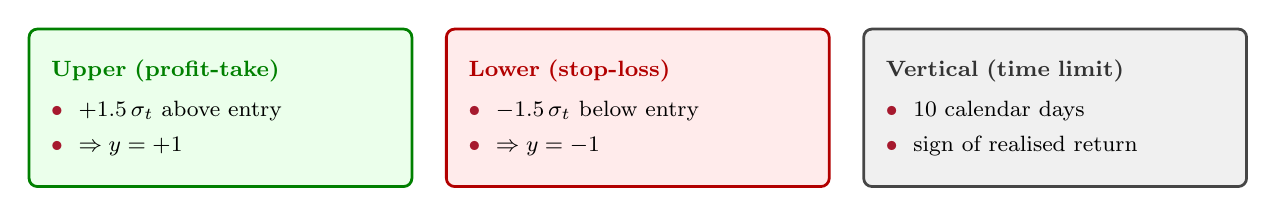
\begin{tikzpicture}[
  bbox/.style={
    rounded corners=3pt, line width=1pt, text width=4.3cm,
    minimum height=2.0cm, align=left, inner sep=8pt, anchor=north,
    font=\footnotesize
  }
]
\node[bbox, draw=green!50!black, fill=green!8] at (-5.3, 0) {%
  \textbf{\color{green!50!black}Upper (profit-take)}\\[5pt]
  \textcolor{isegred}{$\bullet$}~ $+1.5\,\sigma_t$ above entry\\[3pt]
  \textcolor{isegred}{$\bullet$}~ $\Rightarrow y = +1$};

\node[bbox, draw=red!70!black, fill=red!8] at (0, 0) {%
  \textbf{\color{red!70!black}Lower (stop-loss)}\\[5pt]
  \textcolor{isegred}{$\bullet$}~ $-1.5\,\sigma_t$ below entry\\[3pt]
  \textcolor{isegred}{$\bullet$}~ $\Rightarrow y = -1$};

\node[bbox, draw=gray!55!black, fill=gray!12] at (5.3, 0) {%
  \textbf{\color{gray!40!black}Vertical (time limit)}\\[5pt]
  \textcolor{isegred}{$\bullet$}~ 10 calendar days\\[3pt]
  \textcolor{isegred}{$\bullet$}~ sign of realised return};
\end{tikzpicture}
\end{center}

\vspace{-1.7em}

\begin{center}
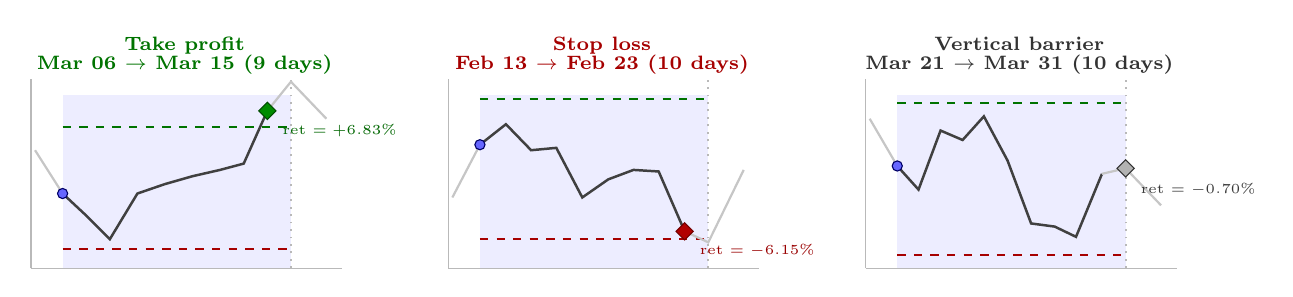
\begin{tikzpicture}[
  font=\tiny,
  xshift=-7.3cm,
  paneltitle/.style={font=\scriptsize\bfseries, align=center},
  axisline/.style={draw=gray!55, line width=0.5pt},
  pathline/.style={draw=black!75, line width=0.9pt},
  greylead/.style={draw=gray!45, line width=0.8pt},
  pt/.style={draw=green!45!black, dashed, line width=0.7pt},
  sl/.style={draw=red!65!black, dashed, line width=0.7pt},
  vb/.style={draw=gray!55, dotted, line width=0.7pt},
  band/.style={fill=blue!7},
  entrydot/.style={circle, fill=blue!60, draw=blue!40!black, inner sep=1.3pt},
  exitup/.style={diamond, fill=green!55!black, draw=green!30!black, inner sep=1.6pt},
  exitdown/.style={diamond, fill=red!70!black, draw=red!45!black, inner sep=1.6pt},
  exitflat/.style={diamond, fill=gray!60, draw=gray!40!black, inner sep=1.6pt}
]

% ============ PANEL 1 : TAKE PROFIT ============
\begin{scope}[xshift=0cm]
  \node[paneltitle, text=green!45!black] at (2.0, 2.75)
    {Take profit\\[-1pt] Mar 06 $\to$ Mar 15 (9 days)};
  \fill[band] (0.45,0.05) rectangle (3.35,2.25);
  \draw[axisline] (0.05,0.05) -- (4.0,0.05);
  \draw[axisline] (0.05,0.05) -- (0.05,2.45);
  \draw[pt] (0.45,1.85) -- (3.35,1.85);
  \draw[sl] (0.45,0.30) -- (3.35,0.30);
  \draw[vb] (3.35,0.05) -- (3.35,2.45);
  \draw[greylead] (0.10,1.55) -- (0.45,1.00);
  \draw[pathline] (0.45,1.00) -- (0.75,0.72) -- (1.05,0.42)
     -- (1.40,1.00) -- (1.75,1.12) -- (2.10,1.22) -- (2.45,1.30)
     -- (2.75,1.38) -- (3.05,2.05);
  \draw[greylead] (3.05,2.05) -- (3.35,2.42) -- (3.80,1.95);
  \node[entrydot] at (0.45,1.00) {};
  \node[exitup]  at (3.05,2.05) {};
  \node[font=\tiny, text=green!40!black, anchor=west] at (3.12,1.80) {ret $= +6.83\%$};
\end{scope}

% ============ PANEL 2 : STOP LOSS ============
\begin{scope}[xshift=5.3cm]
  \node[paneltitle, text=red!65!black] at (2.0, 2.75)
    {Stop loss\\[-1pt] Feb 13 $\to$ Feb 23 (10 days)};
  \fill[band] (0.45,0.05) rectangle (3.35,2.25);
  \draw[axisline] (0.05,0.05) -- (4.0,0.05);
  \draw[axisline] (0.05,0.05) -- (0.05,2.45);
  \draw[pt] (0.45,2.20) -- (3.35,2.20);
  \draw[sl] (0.45,0.42) -- (3.35,0.42);
  \draw[vb] (3.35,0.05) -- (3.35,2.45);
  \draw[greylead] (0.10,0.95) -- (0.45,1.62);
  \draw[pathline] (0.45,1.62) -- (0.78,1.88) -- (1.10,1.55)
     -- (1.42,1.58) -- (1.75,0.95) -- (2.08,1.18) -- (2.40,1.30)
     -- (2.72,1.28) -- (3.05,0.52);
  \draw[greylead] (3.05,0.52) -- (3.35,0.38) -- (3.80,1.30);
  \node[entrydot] at (0.45,1.62) {};
  \node[exitdown] at (3.05,0.52) {};
  \node[font=\tiny, text=red!60!black, anchor=west] at (3.12,0.28) {ret $= -6.15\%$};
\end{scope}

% ============ PANEL 3 : VERTICAL BARRIER ============
\begin{scope}[xshift=10.6cm]
  \node[paneltitle, text=gray!40!black] at (2.0, 2.75)
    {Vertical barrier\\[-1pt] Mar 21 $\to$ Mar 31 (10 days)};
  \fill[band] (0.45,0.05) rectangle (3.35,2.25);
  \draw[axisline] (0.05,0.05) -- (4.0,0.05);
  \draw[axisline] (0.05,0.05) -- (0.05,2.45);
  \draw[pt] (0.45,2.15) -- (3.35,2.15);
  \draw[sl] (0.45,0.22) -- (3.35,0.22);
  \draw[vb] (3.35,0.05) -- (3.35,2.45);
  \draw[greylead] (0.10,1.95) -- (0.45,1.35);
  \draw[pathline] (0.45,1.35) -- (0.72,1.05) -- (1.00,1.80)
     -- (1.28,1.68) -- (1.55,1.98) -- (1.85,1.42) -- (2.15,0.62)
     -- (2.45,0.58) -- (2.72,0.45) -- (3.05,1.25);
  \draw[greylead] (3.05,1.25) -- (3.35,1.32) -- (3.80,0.85);
  \node[entrydot] at (0.45,1.35) {};
  \node[exitflat] at (3.35,1.32) {};
  \node[font=\tiny, text=gray!45!black, anchor=west] at (3.42,1.05) {ret $= -0.70\%$};
\end{scope}

\end{tikzpicture}
\end{center}

\vspace{-0.7em}

\begin{center}
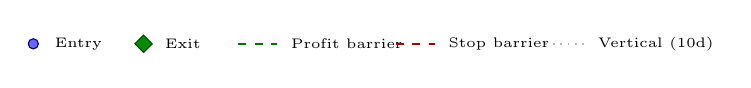
\begin{tikzpicture}[font=\tiny, xshift=-4.2cm]
  \node[circle, fill=blue!60, draw=blue!40!black, inner sep=1.3pt] at (0,0) {};
  \node[anchor=west] at (0.15,0) {Entry};
  \node[diamond, fill=green!55!black, draw=green!30!black, inner sep=1.6pt] at (1.4,0) {};
  \node[anchor=west] at (1.55,0) {Exit};
  \draw[draw=green!45!black, dashed, line width=0.7pt] (2.6,0) -- (3.1,0);
  \node[anchor=west] at (3.15,0) {Profit barrier};
  \draw[draw=red!65!black, dashed, line width=0.7pt] (4.6,0) -- (5.1,0);
  \node[anchor=west] at (5.15,0) {Stop barrier};
  \draw[draw=gray!55, dotted, line width=0.7pt] (6.5,0) -- (7.0,0);
  \node[anchor=west] at (7.05,0) {Vertical (10d)};
\end{tikzpicture}
\end{center}

\vspace{-0.4em}

\begin{itemize}\footnotesize
  \item Vertical hits with $|r| < 2\%$ relabelled to zero (102 events). \textbf{Zero class dropped.}
  \item Final dataset: 1{,}168 binary events.
\end{itemize}

\end{frame}

% =========================================================
%  PHASE I  -  Sample weights (MERGED why + how)
% =========================================================
\begin{frame}{Phase I: Sample weights}
\paramsbox{dim}{lit}{act}{lit}
\vspace{-1.0em}

{\footnotesize \textcolor{isegred}{$\bullet$}~ Price-series observations are \textbf{not i.i.d.}}

\vspace{0.6em}

\begin{columns}[T]
\begin{column}{0.32\textwidth}
{
\setbeamercolor{block title}{bg=blue!22, fg=blue!50!black}
\setbeamercolor{block body}{bg=blue!5, fg=black}
\begin{block}{Overlap}
\centering
\vspace{0.2em}
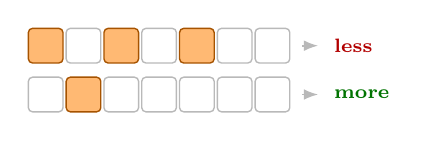
\begin{tikzpicture}[
  day/.style={draw=gray!55, fill=white, rounded corners=1.5pt,
              line width=0.5pt, minimum size=0.44cm, inner sep=0pt},
  trade/.style={draw=orange!65!black, fill=orange!55, rounded corners=1.5pt,
                line width=0.5pt, minimum size=0.44cm, inner sep=0pt}
]
% week 1: 3 trades
\foreach \i/\s in {0/trade, 1/day, 2/trade, 3/day, 4/trade, 5/day, 6/day}{
  \node[\s] at (\i*0.48, 0.62) {};
}
\draw[-{Latex[length=1.8mm]}, line width=0.6pt, draw=gray!55]
  (3.26, 0.62) -- (3.46, 0.62);
\node[font=\scriptsize\bfseries, text=red!70!black, anchor=west] at (3.54, 0.62) {less};

% week 2: 1 trade (day 2)
\foreach \i/\s in {0/day, 1/trade, 2/day, 3/day, 4/day, 5/day, 6/day}{
  \node[\s] at (\i*0.48, 0.0) {};
}
\draw[-{Latex[length=1.8mm]}, line width=0.6pt, draw=gray!55]
  (3.26, 0.0) -- (3.46, 0.0);
\node[font=\scriptsize\bfseries, text=green!45!black, anchor=west] at (3.54, 0.0) {more};
\end{tikzpicture}
\vspace{0.2em}
\end{block}
}
\end{column}

\begin{column}{0.02\textwidth}\hfill\end{column}

\begin{column}{0.30\textwidth}
{
\setbeamercolor{block title}{bg=orange!25, fg=orange!55!black}
\setbeamercolor{block body}{bg=orange!5, fg=black}
\begin{block}{Magnitude}
\centering
\vspace{0.7em}
\footnotesize \textcolor{green!75!black}{$\mathbf{+9\%}$} day $\;\neq\;$ \textcolor{green!35!black}{$\mathbf{+2\%}$} day
\vspace{0.9em}
\end{block}
}
\end{column}

\begin{column}{0.02\textwidth}\hfill\end{column}

\begin{column}{0.30\textwidth}
{
\setbeamercolor{block title}{bg=green!22, fg=green!45!black}
\setbeamercolor{block body}{bg=green!5, fg=black}
\begin{block}{Non-stationarity}
\centering
\vspace{0.3em}
\footnotesize 2016 price action $\;\neq\;$ today's\\[4pt]
{\scriptsize Retail-driven then, institutional now}
\vspace{0.3em}
\end{block}
}
\end{column}
\end{columns}

\vspace{1.0em}

\centering
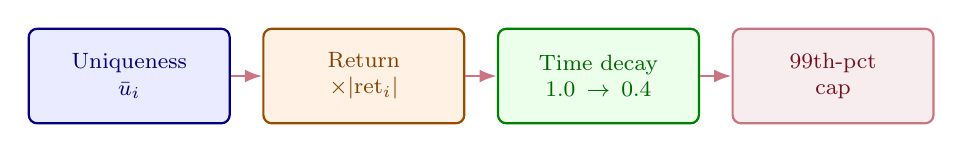
\begin{tikzpicture}[
  wstep/.style={rounded corners=3pt, line width=0.8pt,
                font=\footnotesize, inner sep=5pt,
                align=center, minimum height=1.2cm, text width=2.2cm},
  arr/.style={-{Latex[length=2.2mm]}, line width=1pt, draw=isegred!60}
]
\node[wstep, draw=blue!50!black, fill=blue!8, text=blue!45!black] (s1)
  {Uniqueness\\ \footnotesize $\bar{u}_i$};
\node[wstep, draw=orange!60!black, fill=orange!10, text=orange!50!black,
      right=0.4cm of s1] (s2) {Return\\ \footnotesize $\times |\mathrm{ret}_i|$};
\node[wstep, draw=green!50!black, fill=green!8, text=green!40!black,
      right=0.4cm of s2] (s3) {Time decay\\ \footnotesize $1.0 \to 0.4$};
\node[wstep, draw=isegred!60, fill=isegred!8, text=isegred!70!black,
      right=0.4cm of s3] (s4) {99th-pct\\ cap};
\draw[arr] (s1) -- (s2); \draw[arr] (s2) -- (s3); \draw[arr] (s3) -- (s4);
\end{tikzpicture}

\vspace{0.7em}

{\scriptsize\itshape Steps 1 to 3 follow AFML; the 99th-percentile cap (12 events: COVID, FTX, 2019 rally) is added here.}

\end{frame}

% =========================================================
%  PHASE I  - Feature engineering
% =========================================================
\begin{frame}{Phase I: Feature engineering}
\paramsbox{act}{lit}{lit}{lit}
\vspace{-1.4em}
\centering
{\footnotesize Four feature families, 73 features total. No family privileged a priori.}
\vspace{0.5em}
\begin{columns}[T]
\begin{column}{0.49\textwidth}
{
\setbeamercolor{block title}{bg=blue!22, fg=blue!50!black}
\setbeamercolor{block body}{bg=blue!5, fg=black}
\begin{block}{Technical analysis (25)}
\scriptsize
\begin{itemize}\setlength{\itemsep}{0pt}
  \item Returns and volatility (Garman-Klass, Yang-Zhang).
  \item Momentum (RSI, MACD, ROC).
  \item Volume (OBV, MFI).
  \item Trend ratios (EMA 20/50, 50/200).
\end{itemize}
\end{block}
}
\vspace{0.20em}
{
\setbeamercolor{block title}{bg=violet!25, fg=violet!55!black}
\setbeamercolor{block body}{bg=violet!5, fg=black}
\begin{block}{Autoregressive lag (10)}
\scriptsize
\begin{itemize}\setlength{\itemsep}{0pt}
  \item Log returns at lags $\{1, \ldots, 7, 14, 21, 30\}$.
  \item Own-momentum at short and medium horizons.
\end{itemize}
\end{block}
}
\end{column}
\begin{column}{0.49\textwidth}
{
\setbeamercolor{block title}{bg=orange!25, fg=orange!55!black}
\setbeamercolor{block body}{bg=orange!5, fg=black}
\begin{block}{External (29)}
\scriptsize
\begin{itemize}\setlength{\itemsep}{0pt}
  \item Macro (yields, VIX, DXY, commodities).
  \item Crypto cross-section (ETH/BTC).
  \item On-chain (active addresses, MVRV, hash rate).
\end{itemize}
\end{block}
}
\vspace{0.15em}
{
\setbeamercolor{block title}{bg=green!22, fg=green!45!black}
\setbeamercolor{block body}{bg=green!5, fg=black}
\begin{block}{Mathematical (9)}
\scriptsize
\begin{itemize}\setlength{\itemsep}{0pt}
  \item Information content (Shannon entropy, Lempel-Ziv).
  \item Random walk (Hurst, Lo-MacKinlay).
  \item Structural break (Jarque-Bera, SADF, SMT).
\end{itemize}
\end{block}
}
\end{column}
\end{columns}
\vspace{0.5em}

\begin{center}
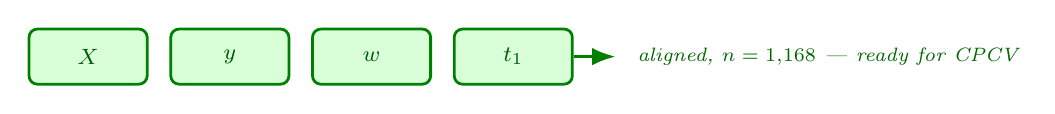
\begin{tikzpicture}[
  donebox/.style={
    draw=green!50!black, fill=green!15, rounded corners=3pt, line width=1pt,
    text=green!35!black, minimum width=1.5cm, minimum height=0.7cm,
    font=\footnotesize\bfseries, inner sep=3pt
  }
]
  \node[donebox] (X)  at (-5.4, 0) {$X$};
  \node[donebox] (y)  at (-3.6, 0) {$y$};
  \node[donebox] (w)  at (-1.8, 0) {$w$};
  \node[donebox] (t1) at ( 0.0, 0) {$t_1$};
  \draw[-{Latex[length=3mm]}, line width=1.2pt, draw=green!50!black]
    (t1.east) -- (1.3, 0);
  \node[font=\scriptsize\itshape, text=green!40!black, anchor=west] at (1.45, 0)
    {aligned, $n = 1{,}168$ \textemdash\ ready for CPCV};
\end{tikzpicture}
\end{center}

\end{frame}

% =========================================================
%  PHASE II  - Intro divider
% =========================================================
\begin{frame}[c]{Phase II: CPCV pipeline}

\centering

{\fontsize{56}{68}\selectfont\bfseries\color{isegred} Phase II}\\[0.5em]
{\Large\itshape CPCV pipeline}\\[2em]


\begin{tikzpicture}[
  pstep/.style={
    draw=isegred, line width=1.2pt,
    fill=isegred!15,
    rounded corners=4pt,
    minimum width=2.4cm, minimum height=1.4cm,
    font=\footnotesize\bfseries, text=isegred,
    align=center, inner sep=4pt
  },
  arrow/.style={
    -{Latex[length=3.5mm, width=3mm]},
    line width=1.4pt, draw=isegred!75
  }
]
\node[pstep] (s1) at (-6, 0) {\shortstack[c]{CPCV\\setup}};
\node[pstep] (s2) at (-3, 0) {\shortstack[c]{Per-fold\\preproc.}};
\node[pstep] (s3) at ( 0, 0) {\shortstack[c]{Optuna\\tuning}};
\node[pstep] (s4) at ( 3, 0) {\shortstack[c]{Train\\6 models}};
\node[pstep] (s5) at ( 6, 0) {Calibrate};

\draw[arrow] (s1) -- (s2);
\draw[arrow] (s2) -- (s3);
\draw[arrow] (s3) -- (s4);
\draw[arrow] (s4) -- (s5);
\end{tikzpicture}

\vspace{2em}

{\normalsize 28 splits, 6 models, 5 seeds, producing 840 test-fold predictions.}

\end{frame}

% =========================================================
%  PHASE II  - Split generation
%  (config top-left, why CPCV top-right, fold viz bottom)
% =========================================================
\begin{frame}{Phase II: CPCV Split generation}
\vspace{-0.6em}

{
\setbeamercolor{block title}{bg=green!22, fg=green!45!black}
\setbeamercolor{block body}{bg=green!5, fg=black}
\begin{block}{Why \textbf{Combinatorial Purged Cross-Validation} over \textbf{walk-forward}?}
\footnotesize
\begin{itemize}\setlength{\itemsep}{4pt}
  \item \textbf{One backtest is one lucky path.} Walk-forward gives a single point estimate; CPCV gives a \emph{distribution} of Sharpes over 7 paths, so we can see how much of the result is chance.
  \item \textbf{Every event gets tested.} In walk-forward the earliest data is never in a test set. Under CPCV each event is tested exactly once per path, so no period is wasted or privileged.
\end{itemize}
\end{block}
}

\vspace{0.6em}

\begin{columns}[T]
\begin{column}{0.05\textwidth}\hfill\end{column}

\begin{column}{0.42\textwidth}
{
\setbeamercolor{block title}{bg=blue!22, fg=blue!50!black}
\setbeamercolor{block body}{bg=blue!5, fg=black}
\begin{block}{Configuration}
\footnotesize
\begin{itemize}\setlength{\itemsep}{2pt}
  \item $N = 8$ groups (146 events each).
  \item $k = 2$ test groups per split.
  \item $\binom{8}{2} = 28$ splits.
  \item 7 backtest paths.
\end{itemize}
\end{block}
}
\end{column}

\begin{column}{0.06\textwidth}\hfill\end{column}

\begin{column}{0.42\textwidth}
{
\setbeamercolor{block title}{bg=orange!25, fg=orange!55!black}
\setbeamercolor{block body}{bg=orange!5, fg=black}
\begin{block}{Leakage controls}
\footnotesize
\begin{itemize}\setlength{\itemsep}{3pt}
  \item \textbf{Purging:} removes training events whose labels resolve inside a test group.
  \item \textbf{Embargo (1\%):} drops the observations immediately after each test group.
\end{itemize}
\end{block}
}
\end{column}

\begin{column}{0.05\textwidth}\hfill\end{column}
\end{columns}

\end{frame}


\begin{frame}{Phase II: One split in detail}
\vspace{-0.4em}

\centering
{\large\bfseries Eight groups, two test, one split at a time}

\vspace{0.8em}

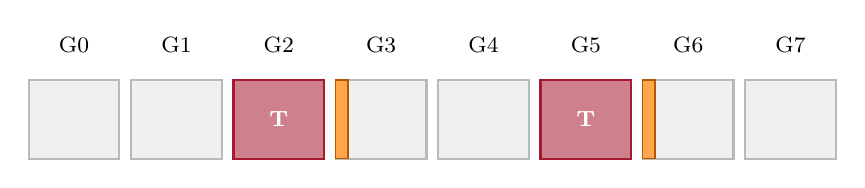
\begin{tikzpicture}[
  gbox/.style={draw=gray!55, fill=gray!12, line width=0.8pt,
               minimum width=1.15cm, minimum height=1.0cm, inner sep=0pt},
  tbox/.style={draw=isegred, fill=isegred!55, line width=0.8pt,
               minimum width=1.15cm, minimum height=1.0cm, inner sep=0pt,
               font=\footnotesize\bfseries, text=white},
  emb/.style={draw=orange!70!black, fill=orange!70, line width=0.5pt,
              minimum width=0.16cm, minimum height=1.0cm, inner sep=0pt},
  lbl/.style={font=\footnotesize, text=black}
]

% group labels
\foreach \i/\n in {0/G0, 1/G1, 2/G2, 3/G3, 4/G4, 5/G5, 6/G6, 7/G7}{
  \node[lbl] at (\i*1.30, 0.95) {\n};
}

% blocks
\node[gbox] at (0*1.30, 0) {};
\node[gbox] at (1*1.30, 0) {};
\node[tbox] at (2*1.30, 0) {T};
\node[gbox] at (3*1.30, 0) {};
\node[gbox] at (4*1.30, 0) {};
\node[tbox] at (5*1.30, 0) {T};
\node[gbox] at (6*1.30, 0) {};
\node[gbox] at (7*1.30, 0) {};

% embargo strips at the left edge of G3 and G6
\node[emb] at (3*1.30 - 0.50, 0) {};
\node[emb] at (6*1.30 - 0.50, 0) {};

\end{tikzpicture}

\vspace{0.7em}

{\large Split 12: test $= \{$G2, G5$\}$}

\vspace{0.4em}

{\footnotesize\color{orange!60!black} Orange strips on G3 and G6: the 1\% embargo after each test block.}

\vspace{0.5em}

{\footnotesize\color{green!45!black} Leakage audit: zero training labels resolve inside their assigned test group.}

\vspace{0.7em}

\begin{itemize}\footnotesize
  \item Training events whose labels resolve inside G2 or G5 are \textbf{purged} before fitting.
  \item Repeating over all $\binom{8}{2} = 28$ combinations yields \textbf{7 non-overlapping backtest paths}.
\end{itemize}

\end{frame}

% =========================================================
%  PHASE II  - Preprocessing 1 (FFD and scaling in two boxes)
% =========================================================
\begin{frame}{Phase II: Preprocessing (FFD \& scaling)}
\vspace{-0.4em}

{
\setbeamercolor{block title}{bg=blue!22, fg=blue!50!black}
\setbeamercolor{block body}{bg=blue!5, fg=black}
\begin{block}{Fractional differentiation (ATR only)}
\footnotesize
\begin{itemize}\setlength{\itemsep}{3pt}
  \item Standard differencing achieves stationarity but destroys long memory; FFD keeps both.
  \item Only the Average True Range fails the per-fold ADF test, so FFD is applied to that feature alone. 
\end{itemize}
\end{block}
}

\vspace{0.3em}

{
\setbeamercolor{block title}{bg=orange!25, fg=orange!55!black}
\setbeamercolor{block body}{bg=orange!5, fg=black}
\begin{block}{Robust scaling (all 73 features)}
\footnotesize
\begin{itemize}\setlength{\itemsep}{3pt}
  \item BTC features have fat tails and regime-break outliers.
  \item Each feature is recentred on its median and rescaled by its interquartile range.
  \item All 73 features are put on a comparable scale without letting extreme moves dominate. Statistics are fit on the training fold only.
\end{itemize}
\vspace{-0.3em}
\[
  x' \;=\; \frac{x - \mathrm{median}(x)}{\mathrm{IQR}(x)}
\]
\vspace{-0.9em}
\end{block}
}

\end{frame}


% =========================================================
%  PHASE II  - Preprocessing (MDA, trimmed for main deck)
% =========================================================
\begin{frame}{Phase II: Feature selection (MDA)}
\vspace{-0.4em}

{
\setbeamercolor{block title}{bg=gray!25, fg=black}
\setbeamercolor{block body}{bg=gray!8, fg=black}
\begin{block}{Mean Decrease in Accuracy}
\footnotesize
\begin{itemize}\setlength{\itemsep}{3pt}
  \item Permute a feature's values, measure the inner-CV accuracy drop. Bigger drop $\Rightarrow$ more informative feature.
  \item Computed with \textbf{two estimators} (Random Forest + Logistic Regression) so no single inductive bias dominates.
\end{itemize}
\end{block}
}

\vspace{0.4em}

\begin{columns}[T]
\begin{column}{0.48\textwidth}
{
\setbeamercolor{block title}{bg=green!22, fg=green!45!black}
\setbeamercolor{block body}{bg=green!5, fg=black}
\begin{block}{Selection rule}
\footnotesize
\begin{itemize}\setlength{\itemsep}{3pt}
  \item Keep features with strictly positive averaged MDA.
  \item Cap at top 20\% ($\approx 14$--$15$ features), floor at 5.
\end{itemize}
\end{block}
}
\end{column}

\begin{column}{0.48\textwidth}
{
\setbeamercolor{block title}{bg=blue!22, fg=blue!50!black}
\setbeamercolor{block body}{bg=blue!5, fg=black}
\begin{block}{Why cap at 14--15?}
\footnotesize
\begin{itemize}\setlength{\itemsep}{3pt}
  \item \textbf{More features} $\Rightarrow$ overfitting; \textbf{fewer} $\Rightarrow$ too little to learn from.
  \item Rule of thumb: aim for $\gtrsim 10$ samples per feature. Here $\approx 686 / 14 \approx 49$, a safe margin.
\end{itemize}
\end{block}
}
\end{column}
\end{columns}

\vspace{0.5em}

\begin{itemize}\footnotesize
  \item \textbf{Exception:} AR Logistic bypasses MDA, using the ten lag columns by name.
\end{itemize}

\end{frame}


% =========================================================
%  PHASE II  - Six models (compacted)
% =========================================================
\begin{frame}{Phase II: Six models}
\vspace{-2.0em}
\begin{columns}[T]
\begin{column}{0.49\textwidth}
{
\setbeamercolor{block title}{bg=blue!22, fg=blue!50!black}
\setbeamercolor{block body}{bg=blue!5, fg=black}
\begin{block}{AR Logistic}
\scriptsize
\begin{itemize}\setlength{\itemsep}{0pt}
  \item Econometric.
  \item Momentum baseline on log-return lags.
  \item Bypasses MDA.
\end{itemize}
\end{block}
}
\vspace{-0.5em}
{
\setbeamercolor{block title}{bg=orange!25, fg=orange!55!black}
\setbeamercolor{block body}{bg=orange!5, fg=black}
\begin{block}{Random Forest}
\scriptsize
\begin{itemize}\setlength{\itemsep}{0pt}
  \item Tree ensemble.
  \item Trees tuned per fold, balanced subsample.
  \item Depth-capped.
\end{itemize}
\end{block}
}
\vspace{-0.5em}
{
\setbeamercolor{block title}{bg=teal!22, fg=teal!55!black}
\setbeamercolor{block body}{bg=teal!5, fg=black}
\begin{block}{LSTM}
\scriptsize
\begin{itemize}\setlength{\itemsep}{0pt}
  \item Neural, temporal.
  \item Single-layer, 14-day sequences.
  \item Captures temporal dependencies.
\end{itemize}
\end{block}
}
\end{column}
\begin{column}{0.49\textwidth}
{
\setbeamercolor{block title}{bg=green!22, fg=green!45!black}
\setbeamercolor{block body}{bg=green!5, fg=black}
\begin{block}{Logistic Regression}
\scriptsize
\begin{itemize}\setlength{\itemsep}{0pt}
  \item Linear ML baseline.
  \item Trained on MDA features.
  \item Isolates nonlinearity contribution.
\end{itemize}
\end{block}
}
\vspace{-0.5em}
{
\setbeamercolor{block title}{bg=violet!25, fg=violet!55!black}
\setbeamercolor{block body}{bg=violet!5, fg=black}
\begin{block}{XGBoost}
\scriptsize
\begin{itemize}\setlength{\itemsep}{0pt}
  \item Gradient boosting.
  \item 500 trees, sequential boosting.
  \item Early stopping on the 20\% holdout.
\end{itemize}
\end{block}
}
\vspace{-0.5em}
{
\setbeamercolor{block title}{bg=isegred!18, fg=isegred}
\setbeamercolor{block body}{bg=isegred!4, fg=black}
\begin{block}{KAN}
\scriptsize
\begin{itemize}\setlength{\itemsep}{0pt}
  \item Neural, interpretable.
  \item Single hidden layer, B-spline edges.
  \item Edges symbolifiable into closed form.
\end{itemize}
\end{block}
}
\end{column}
\end{columns}

\vspace{1.0em}

{\scriptsize\textcolor{isegred}{$\bullet$}~ All 6 trained with AFML sample weights and class-balanced loss.}

{\scriptsize\textcolor{isegred}{$\bullet$}~ 5 enter the per-split \textbf{Optuna} loop (40 trials each); AR Logistic is not tuned.}

\end{frame}

% =========================================================
%  PHASE II  - Calibration (Platt and vector in two boxes)
% =========================================================
\begin{frame}{Phase II: Calibration}
\vspace{-0.4em}

{
\setbeamercolor{block title}{bg=gray!25, fg=black}
\setbeamercolor{block body}{bg=gray!8, fg=black}
\begin{block}{Why calibrate?}
\footnotesize
\begin{itemize}\setlength{\itemsep}{3pt}
  \item Raw classifier scores are not probabilities.
  \item Tree ensembles cluster around $0.4$--$0.6$ and never commit; neural nets are overconfident, pushing outputs below $0.1$ and above $0.9$.
  \item Calibration makes $P(\text{Up}) = 0.7$ mean an empirical 70\% Up rate, which the bet-sizing rule depends on.
\end{itemize}
\end{block}
}
\vspace{0.8em}

\begin{columns}[T]
\begin{column}{0.48\textwidth}
{
\setbeamercolor{block title}{bg=blue!22, fg=blue!50!black}
\setbeamercolor{block body}{bg=blue!5, fg=black}
\begin{block}{Platt scaling}
\centering
\footnotesize
\vspace{-0.2em}
\[
  P_{\text{cal}}(y = 1 \mid z) \;=\; \frac{1}{1 + \exp(\alpha z + \beta)}
\]
\vspace{-0.6em}

\raggedright
\footnotesize \textbf{Used for:} AR Logistic, Logistic Regression, Random Forest, XGBoost.
\end{block}
}
\end{column}

\begin{column}{0.48\textwidth}
{
\setbeamercolor{block title}{bg=green!22, fg=green!45!black}
\setbeamercolor{block body}{bg=green!5, fg=black}
\begin{block}{Vector scaling}
\centering
\footnotesize
\vspace{-0.2em}
\[
  P_{\text{cal}} \;=\; \mathrm{softmax}\!\left( \frac{\mathrm{logits} + b}{T} \right)
\]
\vspace{-0.6em}

\raggedright
\footnotesize \textbf{Used for:} LSTM, KAN.
\end{block}
}
\end{column}
\end{columns}

\end{frame}

% =========================================================
%  PHASE III  - Intro divider
% =========================================================
\begin{frame}[c]{Phase III: Post-CPCV}

\centering

{\fontsize{56}{68}\selectfont\bfseries\color{isegred} Phase III}\\[0.5em]
{\Large\itshape Post-CPCV}\\[2em]


\begin{tikzpicture}[
  topic/.style={
    draw=isegred, line width=1.2pt,
    fill=isegred!15,
    rounded corners=4pt,
    minimum width=5.5cm, minimum height=2cm,
    text=isegred, align=center, inner sep=8pt
  }
]
\node[topic] (t1) at (-3.5, 0) {%
  \shortstack[c]{%
    {\large\bfseries Evaluation metrics}\\
    {\footnotesize\itshape ML / Financial / AFML}%
  }%
};
\node[topic] (t2) at ( 3.5, 0) {%
  \shortstack[c]{%
    {\large\bfseries Symbolic extraction}\\
    {\footnotesize\itshape KAN to closed-form $P(\mathrm{Up})$}%
  }%
};
\end{tikzpicture}

\vspace{2em}

{\normalsize Two layers of analysis on top of the predictions.}

\end{frame}


% =========================================================
%  PHASE III  - Evaluation metrics (only metrics in the paper)
% =========================================================
\begin{frame}{Phase III: Evaluation and symbolic extraction}
\vspace{-0.4em}

{
\setbeamercolor{block title}{bg=blue!22, fg=blue!50!black}
\setbeamercolor{block body}{bg=blue!5, fg=black}
\begin{block}{Evaluation metrics}
\footnotesize
\begin{itemize}\setlength{\itemsep}{3pt}
  \item \textbf{ML metrics} \textemdash\ per-prediction quality: accuracy, F1, AUC-ROC.
  \item \textbf{Financial metrics} \textemdash\ strategy performance: Sharpe ratio, Sortino ratio, maximum drawdown.
  \item \textbf{AFML statistical layer} \textemdash\ overfitting correction: DSR, PBO, DeLong AUC.
\end{itemize}
\vspace{0.2em}
{\scriptsize Models are ranked by \textbf{median path Sharpe}; the other families corroborate rather than decide.}
\end{block}
}

\vspace{0.8em}

{
\setbeamercolor{block title}{bg=green!22, fg=green!45!black}
\setbeamercolor{block body}{bg=green!5, fg=black}
\begin{block}{Symbolic extraction}
\footnotesize
\begin{itemize}\setlength{\itemsep}{3pt}
  \item \textbf{Goal:} convert a trained KAN's learned B-spline edges into a closed-form expression for $P(\mathrm{Up})$.
  \item \textbf{What it returns:}
  \begin{itemize}\setlength{\itemsep}{2pt}
    \item A single closed-form formula for $P(\mathrm{Up} \mid x)$, readable by a human.
    \item Produced whether or not the model predicts well \textemdash\ interpretability is a \emph{separate} deliverable.
  \end{itemize}
\end{itemize}
\end{block}
}

\end{frame}

% =========================================================
%  RESULTS  divider
% =========================================================

\begin{frame}[c]{}
\centering
\vspace*{0.3cm}

{\fontsize{44}{52}\selectfont\bfseries\color{isegred} Results}

\vspace{1.4em}

{\footnotesize Two questions this thesis set out to answer:}

\vspace{0.9em}

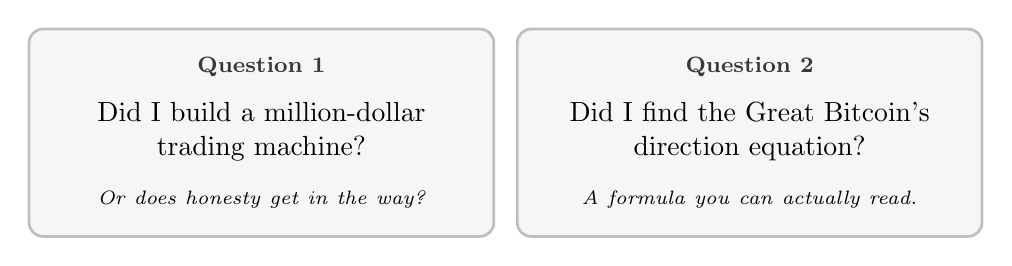
\begin{tikzpicture}[
  qbox/.style={draw=gray!50, fill=gray!7, rounded corners=5pt, line width=1pt,
               text width=5.2cm, minimum height=2.6cm, align=center, inner sep=10pt}
]
\node[qbox] at (-3.1, 0) {%
  {\footnotesize\bfseries\color{gray!45!black}Question 1}\\[6pt]
  {\normalsize Did I build a million-dollar\\ trading machine?}\\[6pt]
  {\scriptsize\itshape Or does honesty get in the way?}};
\node[qbox] at ( 3.1, 0) {%
  {\footnotesize\bfseries\color{gray!45!black}Question 2}\\[6pt]
  {\normalsize Did I find the Great Bitcoin's\\ direction equation?}\\[6pt]
  {\scriptsize\itshape A formula you can actually read.}};
\end{tikzpicture}

\end{frame}

% =========================================================
%  RESULTS  -  Part 1
% =========================================================

\begin{frame}[c]{}
\centering
\vspace*{1.2cm}

{\large We rebuilt the evaluation leakage-free. The honest answer:}

\vspace{1.2em}

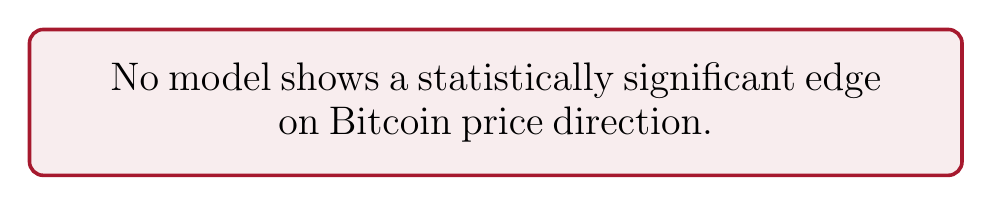
\begin{tikzpicture}
\node[draw=isegred, fill=isegred!8, rounded corners=5pt, line width=1.3pt,
      text width=11cm, align=center, inner sep=12pt]
  {\Large No model shows a statistically significant edge\\[0.15em]
   on Bitcoin price direction.};
\end{tikzpicture}

\vspace{1.4em}

{\footnotesize\itshape Consistent with the semi-strong-form Efficient Market Hypothesis over 2015--2026, and with Chassot \& Audrino (2026): properly-fitted baselines are hard to beat.}

\end{frame}


\begin{frame}{Why: the correction layer}
\vspace{-0.4em}

\centering
{\footnotesize Two independent tests, both pointing the same way.}

\vspace{0.9em}

{
\setbeamercolor{block title}{bg=isegred!15, fg=isegred}
\setbeamercolor{block body}{bg=isegred!4, fg=black}
\begin{block}{Deflated Sharpe Ratio $< 0.95$}
\footnotesize
The best DSR is KAN's which reaches only \textbf{0.247}, far below the 0.95 threshold. Nothing survives the correction.
\end{block}
}

\vspace{0.7em}

{
\setbeamercolor{block title}{bg=isegred!15, fg=isegred}
\setbeamercolor{block body}{bg=isegred!4, fg=black}
\begin{block}{Probability of Backtest Overfitting $> 0.5$}
\footnotesize
The PBO is \textbf{0.657}. Above 0.5 means the in-sample ranking is \emph{anti-informative}: the model that looks best in training tends to underperform out-of-sample.
\end{block}
}

\end{frame}

\begin{frame}{Why KAN ranks first}
\vspace{-0.6em}

{\footnotesize KAN's rank-1 comes from \textbf{how it sizes bets}: abstain when unsure, act only with conviction.}

\vspace{0.8em}

\begin{columns}[c]
\begin{column}{0.44\textwidth}
{
\setbeamercolor{block title}{bg=isegred!15, fg=isegred}
\setbeamercolor{block body}{bg=isegred!4, fg=black}
\begin{block}{Abstains often}
\centering
{\Large\bfseries\color{isegred} 70.1\%}\\[2pt]
{\scriptsize of events \textemdash\ no position when conviction is near 0.5.}
\end{block}
}
\end{column}
\begin{column}{0.08\textwidth}\hfill\end{column}
\begin{column}{0.44\textwidth}
{
\setbeamercolor{block title}{bg=isegred!15, fg=isegred}
\setbeamercolor{block body}{bg=isegred!4, fg=black}
\begin{block}{Bets long}
\centering
{\Large\bfseries\color{isegred} 89.6\%}\\[2pt]
{\scriptsize of non-abstained bets are long.}
\end{block}
}
\end{column}
\end{columns}

\vspace{0.9em}

\begin{center}
\begin{minipage}{0.60\textwidth}
{
\setbeamercolor{block title}{bg=isegred!15, fg=isegred}
\setbeamercolor{block body}{bg=isegred!4, fg=black}
\begin{block}{Shallowest drawdown}
\centering
{\Large\bfseries\color{isegred} $-0.2466$}\\[2pt]
{\scriptsize the least severe median max drawdown among trained models.}
\end{block}
}
\end{minipage}
\end{center}

\vspace{0.9em}

\centering
{\scriptsize Few bets, taken with conviction \textemdash\ the \emph{structural abstention} of Nabar \& Shroff (2023). \textbf{Discipline, not prediction.}}

\end{frame}

\begin{frame}{Which features carried signal?}
\vspace{-0.5em}

{\footnotesize \textbf{Cross-fold MDA selection frequency} across the 28 folds. No feature reaches the stable band ($>80\%$).}

\vspace{0.3em}

\begin{center}
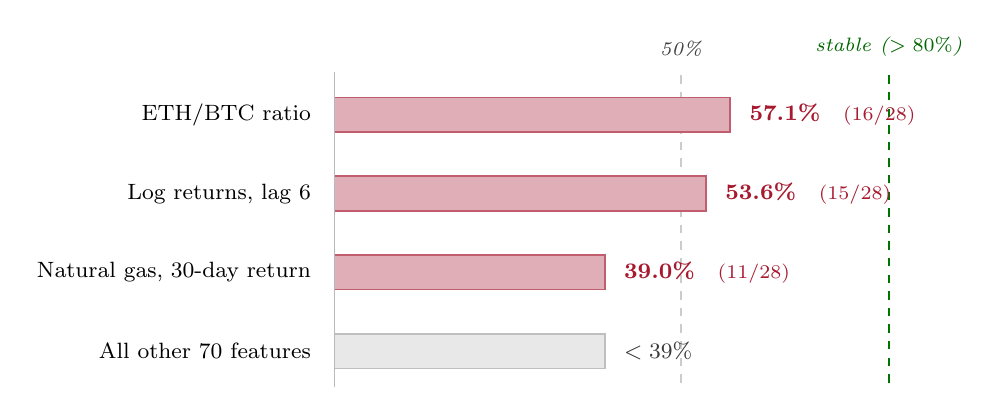
\begin{tikzpicture}[
  xscale=0.088, yscale=1,
  bar/.style={draw=isegred!70, fill=isegred!35, line width=0.6pt},
  dim/.style={draw=gray!50, fill=gray!18, line width=0.6pt},
  lbl/.style={font=\footnotesize, anchor=east, text=black},
  val/.style={font=\footnotesize\bfseries, anchor=west, text=isegred},
  dval/.style={font=\footnotesize, anchor=west, text=gray!45!black},
  zone/.style={font=\scriptsize\itshape, text=gray!50!black}
]

% reference lines
\draw[draw=gray!40, dashed, line width=0.5pt] (50,-0.4) -- (50,3.6);
\node[zone, anchor=south] at (50,3.62) {50\%};
\draw[draw=green!45!black, dashed, line width=0.6pt] (80,-0.4) -- (80,3.6);
\node[zone, anchor=south, text=green!40!black] at (80,3.62) {stable ($>80\%$)};

% bars
\node[lbl] at (-2,3) {ETH/BTC ratio};
\fill[bar] (0,2.78) rectangle (57.1,3.22);
\node[val] at (58.5,3) {57.1\% \, {\scriptsize\mdseries (16/28)}};

\node[lbl] at (-2,2) {Log returns, lag 6};
\fill[bar] (0,1.78) rectangle (53.6,2.22);
\node[val] at (55.0,2) {53.6\% \, {\scriptsize\mdseries (15/28)}};

\node[lbl] at (-2,1) {Natural gas, 30-day return};
\fill[bar] (0,0.78) rectangle (39.0,1.22);
\node[val] at (40.4,1) {39.0\% \, {\scriptsize\mdseries (11/28)}};

\node[lbl] at (-2,0) {All other 70 features};
\fill[dim] (0,-0.22) rectangle (39.0,0.22);
\node[dval] at (40.4,0) {$< 39\%$};

% axis
\draw[draw=gray!55, line width=0.5pt] (0,-0.45) -- (0,3.55);

\end{tikzpicture}
\end{center}

\vspace{0.5em}

\begin{itemize}\footnotesize\setlength{\itemsep}{4pt}
  \item \textbf{Back to the opening question:} \emph{no on-chain feature reaches 50\%}. The ``on-chain free lunch'' does not hold at daily resolution.
  \item The three most-stable features are exactly the three that survive into the symbolic formula.
\end{itemize}

\end{frame}


% =========================================================
%  RESULTS  -  Part 2
% =========================================================
\begin{frame}[c]{}
\centering
\vspace*{1.2cm}

{\large Prediction did not survive. But the second question had a different answer:}

\vspace{1.2em}


\begin{tikzpicture}
\node[draw=isegred, fill=isegred!8, rounded corners=5pt, line width=1.3pt,
      text width=11cm, align=center, inner sep=12pt]
  {\Large The KAN does yield a closed-form\\[0.15em]
   equation for $P(\mathrm{Up})$.};
\end{tikzpicture}

\vspace{1.4em}

{\footnotesize\itshape Interpretability does not depend on the prediction being good.}

\end{frame}

\begin{frame}{What survived: the closed-form formula}
\vspace{-0.4em}

{
\setbeamercolor{block title}{bg=isegred!15, fg=isegred}
\setbeamercolor{block body}{bg=isegred!3, fg=black}
\begin{block}{Closed-form $P(\mathrm{Up} \mid x)$}
\centering
\vspace{-0.4em}
\[
\begin{aligned}
P(\mathrm{Up} \mid x) \;=\; \sigma\Big(\; & \alpha_1 \big[\beta_1\,\text{ETH/BTC} + \beta_2\,\text{lag6}^4 + \beta_3 \tanh(\text{natgas})\big]^2 \\
& +\; \alpha_2 \sin A_2 + \alpha_3 \cos A_3 + \alpha_4 \tanh A_4 + \alpha_0 \;\Big)
\end{aligned}
\]
\vspace{-1.0em}

{\scriptsize $A_2, A_3, A_4$: compositions of the three features. Full form in the appendix.}
\end{block}
}

\vspace{1.0em}

\begin{itemize}\footnotesize\setlength{\itemsep}{5pt}
  \item Split 27, architecture $[3,3,2]$, three input features, 15 of 15 edges symbolified.
  \item 100\% symbolification, median per-edge $R^2$ of 0.990.
  \item Post-symbolic accuracy 51.85\%, below the 56.85\% majority baseline.
\end{itemize}

\end{frame}

% =========================================================
%  LIMITATIONS AND FUTURE WORK (single ranked slide)
% =========================================================
\begin{frame}[c]{The limitation that shaped everything}
\centering

\vspace{0.5em}

{\footnotesize The constraint I kept running into throughout the work:}

\vspace{1.0em}

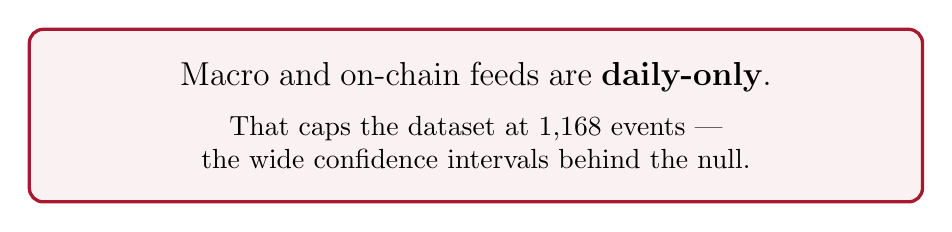
\begin{tikzpicture}
\node[draw=isegred, fill=isegred!6, rounded corners=5pt, line width=1.2pt,
      text width=10.5cm, align=center, inner sep=12pt]
  {\large Macro and on-chain feeds are \textbf{daily-only}.\\[6pt]
   {\normalsize That caps the dataset at 1{,}168 events \textemdash\\ the wide confidence intervals behind the null.}};
\end{tikzpicture}

\vspace{1.2em}

{\large $\downarrow$}

\vspace{0.8em}

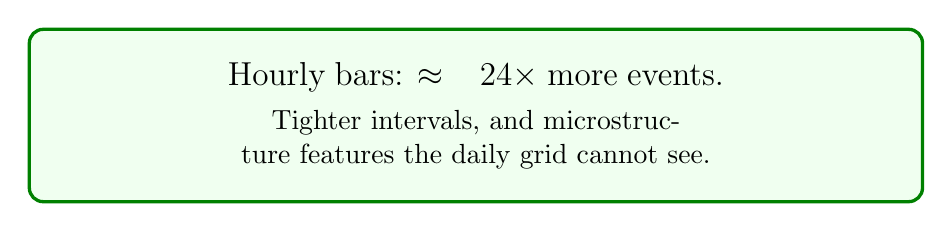
\begin{tikzpicture}
\node[draw=green!50!black, fill=green!6, rounded corners=5pt, line width=1.2pt,
      text width=10.5cm, align=center, inner sep=12pt]
  {\large Hourly bars: $\approx 24\times$ more events.\\[4pt]
   {\normalsize Tighter intervals, and microstructure features the daily grid cannot see.}};
\end{tikzpicture}

\vspace{1.0em}

{\scriptsize\itshape Model capacity and single-fold extraction are the other two limitations \textemdash\ detail in backup.}

\end{frame}


% =========================================================
%  CONCLUSION  (lands on the separability thesis)
% =========================================================
\begin{frame}{Conclusion}
\vspace{-0.8em}

\begin{center}
{\footnotesize Two questions, two honest answers.}
\end{center}

\vspace{0.5em}

\begin{columns}[T]
\begin{column}{0.44\textwidth}
{
\setbeamercolor{block title}{bg=isegred!15, fg=isegred}
\setbeamercolor{block body}{bg=isegred!4, fg=black}
\begin{block}{\small A million-dollar machine?}
\scriptsize
\begin{itemize}\setlength{\itemsep}{3pt}
  \item \textbf{No.}
  \item No model crosses the DSR threshold.
  \item Ranking is adversarial under PBO.
  \item The literature's 80--90\% does not survive.
\end{itemize}
\end{block}
}
\end{column}

\begin{column}{0.08\textwidth}\hfill\end{column}

\begin{column}{0.44\textwidth}
{
\setbeamercolor{block title}{bg=green!22, fg=green!45!black}
\setbeamercolor{block body}{bg=green!5, fg=black}
\begin{block}{\small Bitcoin's direction equation?}
\scriptsize
\begin{itemize}\setlength{\itemsep}{3pt}
  \item \textbf{Yes.}
  \item First closed-form $P(\mathrm{Up})$ from a CPCV-trained KAN.
  \item 100\% symbolification, three readable features.
  \item Smooth and differentiable everywhere.
\end{itemize}
\end{block}
}
\end{column}
\end{columns}

\vspace{1.0em}

{
\setbeamercolor{block title}{bg=yellow!35, fg=black!75}
\setbeamercolor{block body}{bg=yellow!12, fg=black}
\begin{block}{The thesis in one line}
\centering
\small This thesis delivers what a black box cannot: a readable equation for Bitcoin's direction.\\[3pt]
{\scriptsize Interpretability stands on its own, independent of predictive power.}
\end{block}
}

\end{frame}


% =========================================================
%  END PAGE
% =========================================================
\begin{frame}[plain]
  \begin{center}
    \vspace*{1.0cm}
    {\Huge \color{isegred} \textbf{Thank you}}\\[0.8cm]
    {\Large Questions?}\\[1.0cm]
    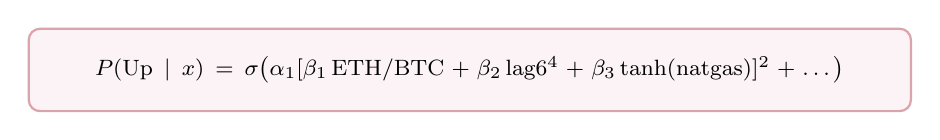
\begin{tikzpicture}
    \node[draw=isegred!40, fill=isegred!5, rounded corners=4pt, line width=0.8pt,
          text width=10.5cm, align=center, inner sep=10pt]
      {\footnotesize $P(\mathrm{Up} \mid x) = \sigma\big(\alpha_1[\beta_1\,\text{ETH/BTC} + \beta_2\,\text{lag6}^4 + \beta_3\tanh(\text{natgas})]^2 + \ldots\big)$};
    \end{tikzpicture}\\[1.0cm]
    \includegraphics[height=1.2cm]{ISEG_logo.png}\\[0.5em]
    {\small Petr Terletskiy \,\textbar\, ISEG / ULisboa}
  \end{center}
\end{frame}


% =========================================================
% =========================================================
%                    BACKUP SLIDES
% =========================================================
% =========================================================

\begin{frame}[c]{}
\centering
\vspace*{2cm}
{\fontsize{40}{48}\selectfont\bfseries\color{isegred} Backup}\\[0.5em]
{\large\itshape Supporting detail for questions}
\end{frame}


% =========================================================
%  BACKUP  -  Phase I: Data (sources)
% =========================================================
\begin{frame}{Backup: Data sources}
\vspace{-0.6em}

\begin{columns}[T]
\begin{column}{0.45\textwidth}
{
\setbeamercolor{block title}{bg=blue!22, fg=blue!50!black}
\setbeamercolor{block body}{bg=blue!5, fg=black}
\begin{block}{Instrument}
\footnotesize
\begin{itemize}
  \item \textbf{Asset:} BTC-USD.
  \item \textbf{Type:} Daily OHLCV bars.
  \item \textbf{Range:} 2014-11-01 to 2026-05-09.
  \item \textbf{Count:} 4{,}208 daily bars.
\end{itemize}
\end{block}
}
\end{column}
\begin{column}{0.06\textwidth}\hfill\end{column}
\begin{column}{0.45\textwidth}
{
\setbeamercolor{block title}{bg=green!22, fg=green!45!black}
\setbeamercolor{block body}{bg=green!5, fg=black}
\begin{block}{Sources}
\footnotesize
\begin{itemize}
  \item Yahoo Finance: BTC OHLCV and macro.
  \item FRED: yield curves and dollar index.
  \item CoinMetrics: ETH/BTC and on-chain metrics.
\end{itemize}
\end{block}
}
\end{column}
\end{columns}

\vfill

\begin{center}
  \includegraphics[height=2.8cm]{btc_usd_close_price.png}\\[2pt]
  {\scriptsize\itshape BTC-USD daily close.}
\end{center}
\end{frame}


% =========================================================
%  BACKUP  -  Phase I: Daily volatility (EWMA)
% =========================================================
\begin{frame}{Backup: Daily volatility (EWMA)}
\vspace{-1.2em}

\begin{block}{Calculation}
\centering
EWMA of squared log returns, recursive form:
\[
  \sigma_t^2 \;=\; (1-\alpha)\,\sigma_{t-1}^2 \;+\; \alpha\,r_t^2,
  \qquad \alpha = \tfrac{2}{\mathrm{span}+1} = \tfrac{2}{51}
\]
\end{block}

\vspace{0.3em}

\begin{columns}[T]
\begin{column}{0.45\textwidth}
{
\setbeamercolor{block title}{bg=blue!22, fg=blue!50!black}
\setbeamercolor{block body}{bg=blue!5, fg=black}
\begin{block}{Why span $= 50$?}
\footnotesize
\begin{itemize}
  \item Shortened from AFML's default of 100 (calibrated to equities).
  \item Tracks BTC's faster regime transitions (halving cycles, regulatory shocks).
  \item Half-life $\approx$ 17 days, memory of about two trading weeks.
\end{itemize}
\end{block}
}
\end{column}
\begin{column}{0.06\textwidth}\hfill\end{column}
\begin{column}{0.45\textwidth}
{
\setbeamercolor{block title}{bg=orange!25, fg=orange!55!black}
\setbeamercolor{block body}{bg=orange!5, fg=black}
\begin{block}{Downstream uses}
\footnotesize
\begin{itemize}
  \item \textbf{CUSUM threshold:} $h = 1.0\,\bar{\sigma}$, constant signal-to-noise.
  \item \textbf{TBL barriers:} horizontal widths scale with $\sigma_t$ at each event.
\end{itemize}
\end{block}
}
\end{column}
\end{columns}
\end{frame}


% =========================================================
%  BACKUP  -  Phase I: CUSUM truncation date detail
% =========================================================
\begin{frame}{Backup: CUSUM event-window start}
\vspace{-0.4em}

\begin{itemize}\footnotesize
  \item The accumulators run on the full raw return series from 2014-11-01.
  \item But the \textbf{event-firing window is truncated to start 2015-08-08}, set by two constraints:
  \begin{itemize}\footnotesize
    \item the 50/200 EMA ratio needs 200 calendar days to populate;
    \item the ETH-USD series (feeding the ETH/BTC feature) begins 2015-08-08.
  \end{itemize}
  \item Events surviving truncation reflect the genuine state of the cumulative drift at firing, \textbf{not} a reset on the start date.
\end{itemize}

\vspace{0.5em}
\centering
{\footnotesize Output: 1{,}270 candidate events entering triple-barrier labelling.}
\end{frame}


% =========================================================
%  BACKUP  -  CUSUM threshold choice
% =========================================================
\begin{frame}{Backup: The CUSUM threshold $h$}
\vspace{-0.4em}

\begin{itemize}\footnotesize\setlength{\itemsep}{4pt}
  \item $h = 1.0 \times \bar{\sigma}$, where $\bar{\sigma}$ is the mean EWMA daily volatility over the sample.
  \item Scaling by volatility means the filter fires at \textbf{constant signal-to-noise}: the same threshold is harder to cross in calm regimes and easier in volatile ones, which is the intended behaviour.
  \item The multiplier was chosen to balance two competing pressures:
  \begin{itemize}\footnotesize
    \item a lower $h$ fires more events but admits noise, diluting the post-TBL class composition;
    \item a higher $h$ yields cleaner events but shrinks the sample below what the models can learn from.
  \end{itemize}
\end{itemize}

\vspace{0.6em}
\centering
{\footnotesize At $h = 1.0\,\bar{\sigma}$: \textbf{1{,}270 events}, $\approx 30\%$ of the 4{,}208 daily bars.}
\end{frame}


% =========================================================
%  BACKUP  -  Phase I: Sample weights mechanics
% =========================================================
\begin{frame}{Backup: Sample-weight mechanics}
\vspace{-0.6em}

\begin{columns}[T]
\begin{column}{0.58\textwidth}
\footnotesize
\begin{enumerate}\setlength{\itemsep}{2pt}
  \item \textbf{Concurrency $c_t$:} overlapping open positions on day $t$.
  \item \textbf{Uniqueness $\bar{u}_i$:} mean $1/c_t$ over the event window.
  \item \textbf{Return scaling:} $w_i = \bar{u}_i \times |\mathrm{ret}_i|$.
  \item \textbf{Time decay:} linear $1.0 \to 0.4$ (newest to oldest).
  \item \textbf{99th-pct cap:} $\approx 2.862$, 12 events hit it.
\end{enumerate}
\end{column}

\begin{column}{0.01\textwidth}\hfill\end{column}

\begin{column}{0.37\textwidth}
{
\setbeamercolor{block title}{bg=orange!25, fg=orange!55!black}
\setbeamercolor{block body}{bg=orange!5, fg=black}
\begin{block}{Provenance}
\scriptsize
\begin{itemize}\setlength{\itemsep}{3pt}
  \item Steps 1 to 4 follow AFML.
  \item The 99th-percentile cap is added here.
\end{itemize}
\end{block}
}
\end{column}
\end{columns}

\vspace{-0.8em}

\begin{center}
  \includegraphics[width=0.85\textwidth]{sample_weights.png}\\[2pt]
  {\scriptsize\itshape Weight distribution and weights over time.}
\end{center}

\end{frame}


% =========================================================
%  BACKUP  -  Phase I: Data alignment (X, y, w, t1)
% =========================================================
\begin{frame}{Backup: Data alignment}
\vspace{-1.0em}

\begin{columns}[T]
\begin{column}{0.45\textwidth}
{
\setbeamercolor{block title}{bg=blue!22, fg=blue!50!black}
\setbeamercolor{block body}{bg=blue!5, fg=black}
\begin{block}{$X$ \textemdash\ feature matrix}
\footnotesize
\begin{minipage}[t][1.4cm][t]{\linewidth}
$1{,}168 \times 73$; four feature families combined (technical, autoregressive, external, mathematical).
\end{minipage}
\end{block}
}
\vspace{0.4em}
{
\setbeamercolor{block title}{bg=green!22, fg=green!45!black}
\setbeamercolor{block body}{bg=green!5, fg=black}
\begin{block}{$y$ \textemdash\ binary labels}
\footnotesize
\begin{minipage}[t][1.4cm][t]{\linewidth}
$\{-1,+1\}$; \textbf{56.85\% Up}, \textbf{43.15\% Down}; the zero class was dropped.
\end{minipage}
\end{block}
}
\end{column}
\begin{column}{0.06\textwidth}\hfill\end{column}
\begin{column}{0.45\textwidth}
{
\setbeamercolor{block title}{bg=orange!25, fg=orange!55!black}
\setbeamercolor{block body}{bg=orange!5, fg=black}
\begin{block}{$w$ \textemdash\ sample weights}
\footnotesize
\begin{minipage}[t][1.4cm][t]{\linewidth}
AFML weighting (uniqueness, return, decay) plus a 99th-percentile cap added here.
\end{minipage}
\end{block}
}
\vspace{0.4em}
{
\setbeamercolor{block title}{bg=violet!25, fg=violet!55!black}
\setbeamercolor{block body}{bg=violet!5, fg=black}
\begin{block}{$t_1$ \textemdash\ barrier-touch timestamps}
\footnotesize
\begin{minipage}[t][1.4cm][t]{\linewidth}
Calendar day each position closed; drives CPCV purging and the embargo.
\end{minipage}
\end{block}
}
\end{column}
\end{columns}

\vspace{1.5em}
\centering
{\footnotesize \textbf{Result:} event-indexed series at $n = 1{,}168$, ready for CPCV.}
\end{frame}


% =========================================================
%  BACKUP  -  Phase II: MDA multi-model mechanics
% =========================================================
\begin{frame}{Backup: Multi-model MDA mechanics}
\vspace{-0.6em}

{
\setbeamercolor{block title}{bg=blue!22, fg=blue!50!black}
\setbeamercolor{block body}{bg=blue!5, fg=black}
\begin{block}{Why two estimators?}
\footnotesize
\begin{itemize}\setlength{\itemsep}{1pt}
  \item A single estimator imposes its own inductive bias on the ranking.
  \item \textbf{Random Forest} (500 trees) captures nonlinear interactions.
  \item \textbf{Logistic Regression} captures linear marginal effects.
  \item Scores are averaged as a \textbf{raw mean} $\bar{m}_j = (m^{\mathrm{RF}}_j + m^{\mathrm{LR}}_j)/2$.
  \item RF drops F1 by 0.005--0.05 per feature; LR an order of magnitude smaller, so \textbf{RF anchors the ranking}, LR acts as a soft tiebreaker near the zero boundary.
\end{itemize}
\end{block}
}

\vspace{0.3em}
\centering
{\footnotesize Computed inside a 3-fold purged inner CV using the same $t_1$-overlap conditions as the outer CPCV.}
\end{frame}


% =========================================================
%  BACKUP  -  FFD differencing order
% =========================================================
\begin{frame}{Backup: Choosing the differencing order $d^\ast$}
\vspace{-0.4em}

\begin{itemize}\footnotesize\setlength{\itemsep}{4pt}
  \item Sweep $d \in [0, 1]$ in steps of $0.05$; for each $d$, difference the series and run an ADF test.
  \item Take the \textbf{smallest} $d^\ast$ that achieves stationarity at $\alpha = 0.05$, preserving as much memory as possible.
  \item Fallback to $d = 1.0$ (standard differencing) if no fractional order passes.
  \item Fitted \textbf{per fold} on training data only, so the choice never sees test observations.
\end{itemize}

\vspace{0.6em}

{
\setbeamercolor{block title}{bg=green!22, fg=green!45!black}
\setbeamercolor{block body}{bg=green!5, fg=black}
\begin{block}{Stability across 140 estimates}
\footnotesize
$\bar{d}^\ast = 0.198$, $\sigma_{d^\ast} = 0.085$. Low turnover in $d^\ast$ contrasts with the high turnover in \emph{which features} are selected: the stationarity property is stable across regimes even as the signal-to-noise composition shifts.
\end{block}
}
\end{frame}


% =========================================================
%  BACKUP  -  Phase II: Optuna tuning loop
% =========================================================
\begin{frame}{Backup: Hyperparameter tuning (Optuna)}
\vspace{-0.5em}

\begin{columns}[T]
\begin{column}{0.46\textwidth}
\footnotesize
\begin{enumerate}\setlength{\itemsep}{2pt}
  \item \textbf{Propose} hparams via the TPE sampler (learns from past trials).
  \item \textbf{Evaluate} on a 3-fold purged inner CV, scoring by log-loss.
  \item \textbf{Prune} early if the intermediate score is below the running median (MedianPruner).
  \item Repeat $\times 40$, then \textbf{refit} the best trial on the full training fold.
\end{enumerate}
\vspace{0.3em}
{\scriptsize 5 tuned models; AR Logistic is fixed. Total: $28 \times 5 \times 40 = 5{,}600$ trials.}
\end{column}
\begin{column}{0.04\textwidth}\hfill\end{column}
\begin{column}{0.46\textwidth}
\centering
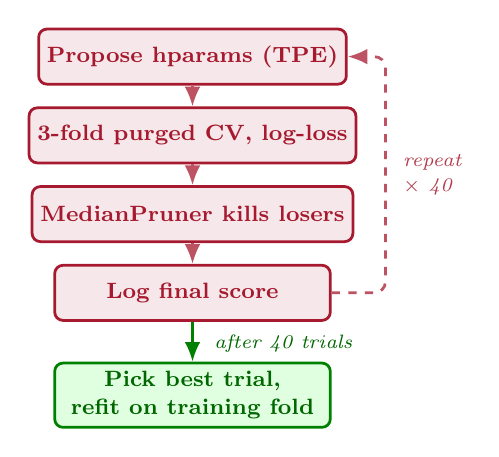
\begin{tikzpicture}[
  fbox/.style={
    draw=isegred, line width=1pt, rounded corners=3pt,
    fill=isegred!10, text=isegred,
    minimum width=3.5cm, minimum height=0.7cm,
    font=\footnotesize\bfseries, align=center, inner sep=3pt
  },
  pickbox/.style={
    draw=green!50!black, line width=1pt, rounded corners=3pt,
    fill=green!12, text=green!40!black,
    minimum width=3.5cm, minimum height=0.7cm,
    font=\footnotesize\bfseries, align=center, inner sep=3pt
  },
  arrow/.style={-{Latex[length=2.5mm, width=2mm]}, line width=1pt, draw=isegred!75},
  loop/.style={-{Latex[length=2.5mm, width=2mm]}, line width=1pt, draw=isegred!75, dashed},
  finalarrow/.style={-{Latex[length=2.5mm, width=2mm]}, line width=1pt, draw=green!50!black}
]
\node[fbox] (a) at (0, 2.0)  {Propose hparams (TPE)};
\node[fbox] (b) at (0, 1.0)  {3-fold purged CV, log-loss};
\node[fbox] (c) at (0, 0.0)  {MedianPruner kills losers};
\node[fbox] (d) at (0,-1.0)  {Log final score};
\node[pickbox] (e) at (0,-2.3) {\shortstack[c]{Pick best trial,\\refit on training fold}};
\draw[arrow] (a) -- (b);
\draw[arrow] (b) -- (c);
\draw[arrow] (c) -- (d);
\draw[loop, rounded corners=4pt] (d.east) -- (2.45,-1.0) -- (2.45,2.0) -- (a.east);
\node[font=\scriptsize\itshape, color=isegred!85, anchor=west] at (2.55, 0.5) {\shortstack[l]{repeat\\$\times$ 40}};
\draw[finalarrow] (d) -- (e);
\node[font=\scriptsize\itshape, color=green!40!black, anchor=west] at (0.15, -1.65) {after 40 trials};
\end{tikzpicture}
\end{column}
\end{columns}
\end{frame}


% =========================================================
%  BACKUP  -  Two Random Forests
% =========================================================
\begin{frame}{Backup: Two Random Forests, two roles}
\vspace{-0.4em}

\begin{columns}[T]
\begin{column}{0.45\textwidth}
{
\setbeamercolor{block title}{bg=blue!22, fg=blue!50!black}
\setbeamercolor{block body}{bg=blue!5, fg=black}
\begin{block}{MDA-side RF}
\footnotesize
Fixed at \textbf{500 trees}. Used only inside feature selection to score permutation importance. Not tuned.
\end{block}
}
\end{column}
\begin{column}{0.06\textwidth}\hfill\end{column}
\begin{column}{0.45\textwidth}
{
\setbeamercolor{block title}{bg=orange!25, fg=orange!55!black}
\setbeamercolor{block body}{bg=orange!5, fg=black}
\begin{block}{Benchmarked RF}
\footnotesize
\texttt{n\_estimators} \textbf{tuned per fold} over $\{100,150,200,250\}$. One of the six compared models.
\end{block}
}
\end{column}
\end{columns}

\vspace{1.5em}
\centering
{\footnotesize Same algorithm, different jobs: a fixed measurement tool vs.\ a tuned competitor.}
\end{frame}


% =========================================================
%  BACKUP  -  Calibration partition (merged with 80/20 rationale)
% =========================================================
\begin{frame}{Backup: The calibration partition}
\vspace{-0.4em}

\begin{itemize}\footnotesize\setlength{\itemsep}{4pt}
  \item \textbf{Per-fold two-way split:} 80\% model-training / 20\% holdout. At $N = 8$ that is roughly 686 / 172 events.
  \item The holdout does double duty: \textbf{early-stopping signal} (XGBoost, LSTM, KAN) \emph{and} \textbf{calibrator fit}.
  \item Platt scaling fitted on the holdout with no regularisation; vector scaling optimised by L-BFGS-B from $T = 1$, $b = 0$, with $T \in [0.05, 20]$ and $b \in [-5, 5]$.
\end{itemize}

\vspace{1.5em}

{
\setbeamercolor{block title}{bg=orange!25, fg=orange!55!black}
\setbeamercolor{block body}{bg=orange!5, fg=black}
\begin{block}{Why not a three-way split?}
\footnotesize
This is a mild coupling: the calibrator sees logits from a model selected on the same partition. A third dedicated calibration slice would shrink model-training to $\approx 600$ events, risking underfitting the KAN and LSTM. At 1{,}168 total events, protecting the training partition mattered more than eliminating the coupling.
\end{block}
}
\end{frame}


% =========================================================
% ---------  EVALUATION METRICS GROUP  --------------------
% =========================================================

% =========================================================
%  BACKUP  -  Full evaluation metric set
% =========================================================
\begin{frame}{Backup: Full evaluation metric set}
\vspace{-0.5em}
\centering
{\footnotesize Computed on the 840 test-fold predictions per model.}
\vspace{0.6em}

\begin{columns}[T]
\begin{column}{0.03\textwidth}\hfill\end{column}
\begin{column}{0.28\textwidth}
{
\setbeamercolor{block title}{bg=blue!22, fg=blue!50!black}
\setbeamercolor{block body}{bg=blue!5, fg=black}
\begin{block}{ML metrics}
\scriptsize
\begin{itemize}\setlength{\itemsep}{1pt}
  \item Accuracy (raw and sample-weighted)
  \item F1 score
  \item Log-loss
  \item AUC-ROC
\end{itemize}
\end{block}
}
\end{column}
\begin{column}{0.04\textwidth}\hfill\end{column}
\begin{column}{0.28\textwidth}
{
\setbeamercolor{block title}{bg=green!22, fg=green!45!black}
\setbeamercolor{block body}{bg=green!5, fg=black}
\begin{block}{Financial metrics}
\scriptsize
\begin{itemize}\setlength{\itemsep}{1pt}
  \item Sharpe ratio (per path)
  \item Sortino ratio
  \item Cumulative return
  \item Maximum drawdown
  \item Win rate, profit factor
\end{itemize}
\end{block}
}
\end{column}
\begin{column}{0.04\textwidth}\hfill\end{column}
\begin{column}{0.28\textwidth}
{
\setbeamercolor{block title}{bg=orange!25, fg=orange!55!black}
\setbeamercolor{block body}{bg=orange!5, fg=black}
\begin{block}{AFML layer}
\scriptsize
\begin{itemize}\setlength{\itemsep}{1pt}
  \item DSR (Deflated Sharpe)
  \item PBO (Backtest Overfitting)
  \item DeLong AUC (pairwise)
\end{itemize}
\end{block}
}
\end{column}
\begin{column}{0.03\textwidth}\hfill\end{column}
\end{columns}

\vspace{1.5em}
\centering
{\footnotesize Ranking is by \textbf{median path Sharpe}; the other families corroborate rather than decide.}
\end{frame}


% =========================================================
%  BACKUP  -  Why sqrt(365) annualisation
% =========================================================
\begin{frame}{Backup: Why $\sqrt{365}$ annualisation?}
\vspace{-0.4em}

\begin{itemize}\footnotesize
  \item Returns are sampled at CUSUM \emph{events} ($\approx 109$/year), not daily bars.
  \item Annualising at the event rate ($\sqrt{109} \approx 10.4$) would roughly \emph{halve} every Sharpe.
  \item $\sqrt{365}$ keeps Sharpes on the daily-equivalent scale the finance literature uses.
\end{itemize}

\vspace{0.5em}
{
\setbeamercolor{block title}{bg=green!22, fg=green!45!black}
\setbeamercolor{block body}{bg=green!5, fg=black}
\begin{block}{The key point: rankings are invariant}
\footnotesize
The DSR de-annualises by the \emph{same} $\sqrt{365}$ before the multiple-testing correction. So DSR verdicts and model rankings do \textbf{not} depend on the annualisation convention.
\end{block}
}
\end{frame}


% =========================================================
%  BACKUP  -  DSR counts 6 models, not 5600 trials
% =========================================================
\begin{frame}{Backup: DSR counts 6 models, not 5{,}600 trials}
\vspace{-0.4em}

\begin{itemize}\footnotesize
  \item The tuning loop runs $28 \times 5 \times 40 = 5{,}600$ Optuna trials in total.
  \item But Optuna trials produce \textbf{inner-CV log-loss}, not test-fold Sharpe.
  \item They never enter the strategy population the DSR corrects over.
\end{itemize}

\vspace{0.5em}
{
\setbeamercolor{block title}{bg=green!22, fg=green!45!black}
\setbeamercolor{block body}{bg=green!5, fg=black}
\begin{block}{The DSR multiple-testing count is 6}
\footnotesize
The six \emph{models} are the candidate strategies. Hyperparameter search is nested \emph{inside} each fold and is invisible to the DSR, the nested-CV discipline of AFML Chapter 7.
\end{block}
}
\end{frame}


% =========================================================
%  BACKUP  -  Statistical correction layer (full 3-box)
% =========================================================
\begin{frame}{Backup: DSR, PBO, DeLong detail}
\vspace{-0.6em}

\begin{columns}[T]
\begin{column}{0.03\textwidth}\hfill\end{column}
\begin{column}{0.28\textwidth}
{
\setbeamercolor{block title}{bg=blue!22, fg=blue!50!black}
\setbeamercolor{block body}{bg=blue!5, fg=black}
\begin{block}{DSR}
\footnotesize
\textit{Multiple-testing correction}
\begin{itemize}\setlength{\itemsep}{0pt}
  \item Adjusts Sharpe for six candidates.
  \item Threshold 0.95 $=$ 5\% significance.
  \item \textbf{KAN: 0.247}.
  \item \textbf{No model crosses 0.95.}
\end{itemize}
\end{block}
}
\end{column}
\begin{column}{0.04\textwidth}\hfill\end{column}
\begin{column}{0.28\textwidth}
{
\setbeamercolor{block title}{bg=orange!25, fg=orange!55!black}
\setbeamercolor{block body}{bg=orange!5, fg=black}
\begin{block}{PBO}
\footnotesize
\textit{Backtest overfitting}
\begin{itemize}\setlength{\itemsep}{0pt}
  \item \textbf{Baseline 0.657} (adversarial).
  \item RF is the anchor.
  \item LR destabilises ($\Delta = -0.286$).
  \item Dropping KAN: 0.543.
\end{itemize}
\end{block}
}
\end{column}
\begin{column}{0.04\textwidth}\hfill\end{column}
\begin{column}{0.28\textwidth}
{
\setbeamercolor{block title}{bg=green!22, fg=green!45!black}
\setbeamercolor{block body}{bg=green!5, fg=black}
\begin{block}{DeLong AUC}
\footnotesize
\textit{Pairwise discriminability}
\begin{itemize}\setlength{\itemsep}{0pt}
  \item \textbf{2 of 15 pairs} significant.
  \item AR Log vs XGB ($p=0.0427$).
  \item RF vs XGB ($p=0.0318$).
  \item KAN indistinguishable from all.
\end{itemize}
\end{block}
}
\end{column}
\begin{column}{0.03\textwidth}\hfill\end{column}
\end{columns}

\vspace{1.0em}

\begin{itemize}\scriptsize\setlength{\itemsep}{4pt}
  \item \textbf{DSR:} asks whether a Sharpe ratio this high could have appeared by luck, given six models were tried, and returns the probability that the result is real rather than the best draw from noise.
  \item \textbf{PBO:} asks whether picking the best model in-sample actually helps out-of-sample; above 0.5 the answer is no, the in-sample winner tends to underperform.
\end{itemize}

\vspace{0.5em}
\centering
{\footnotesize Both significant pairs have XGBoost as the lower-AUC half.}
\end{frame}


% =========================================================
%  BACKUP  -  Full DeLong pairwise table
% =========================================================
\begin{frame}{Backup: DeLong pairwise AUC (key pairs)}
\vspace{-0.5em}
\begin{center}
\renewcommand{\arraystretch}{1.15}
\scriptsize
\begin{tabular}{l r r r c}
\toprule
\textbf{Pair} & $\mathbf{\Delta AUC}$ & $\mathbf{z}$ & $\mathbf{p}$ & \textbf{Sig.} \\
\midrule
AR Log vs XGBoost   & $+0.0175$ & $2.03$  & 0.0427 & \textbf{yes} \\
RF vs XGBoost       & $+0.0127$ & $2.15$  & 0.0318 & \textbf{yes} \\
XGBoost vs KAN      & $-0.0121$ & $-1.69$ & 0.0916 & \\
Logistic vs XGBoost & $+0.0143$ & $1.77$  & 0.0763 & \\
AR Log vs LSTM      & $+0.0100$ & $0.99$  & 0.3213 & \\
\midrule
\multicolumn{5}{c}{\scriptsize All 10 other pairs: $p > 0.48$, none significant.} \\
\bottomrule
\end{tabular}
\end{center}
\vspace{0.3em}
{\scriptsize Pooled across 28 splits, seed-averaged per cell. \textbf{No KAN pair is significant.}}
\end{frame}


% =========================================================
%  BACKUP  -  Leave-one-out PBO
% =========================================================
\begin{frame}{Backup: Leave-one-out PBO}
\vspace{-0.5em}
\centering
{\footnotesize Baseline six-model PBO $= 0.657$. Each row drops one model and recomputes.}
\vspace{0.5em}
\begin{center}
\renewcommand{\arraystretch}{1.3}
\scriptsize
\begin{tabular}{l r r}
\toprule
\textbf{Model dropped} & \textbf{5-model PBO} & $\mathbf{\Delta}$ \\
\midrule
Logistic Regression & 0.371 & $-0.286$ \\
AR Logistic         & 0.457 & $-0.200$ \\
LSTM                & 0.457 & $-0.200$ \\
XGBoost             & 0.543 & $-0.114$ \\
KAN                 & 0.543 & $-0.114$ \\
Random Forest       & 0.657 & $+0.000$ \\
\bottomrule
\end{tabular}
\end{center}
\vspace{0.4em}
\begin{itemize}\scriptsize
  \item \textbf{Random Forest is the anchor:} its removal leaves PBO unchanged.
  \item \textbf{Logistic Regression is the largest destabiliser.}
\end{itemize}
\end{frame}


% =========================================================
%  BACKUP  -  Calibration first-moment audit
% =========================================================
\begin{frame}{Backup: Calibration first-moment audit}
\vspace{-0.5em}
\centering
{\footnotesize Mean $P(\mathrm{Up})$ vs.\ empirical base rate $0.5685$; tolerance $\pm 0.03$.}
\vspace{0.5em}
\begin{center}
\renewcommand{\arraystretch}{1.25}
\scriptsize
\begin{tabular}{l r r c}
\toprule
\textbf{Model} & \textbf{Mean $P(\mathrm{Up})$} & $\mathbf{\Delta}$ & \textbf{In tol.} \\
\midrule
AR Logistic         & 0.5440 & $-0.0245$ & yes \\
Logistic Regression & 0.5506 & $-0.0179$ & yes \\
Random Forest       & 0.5418 & $-0.0267$ & yes \\
XGBoost             & 0.5314 & $-0.0371$ & \textbf{no} \\
LSTM                & 0.5497 & $-0.0187$ & yes \\
KAN                 & 0.5421 & $-0.0263$ & yes \\
\bottomrule
\end{tabular}
\end{center}
\vspace{0.3em}
{\scriptsize Only XGBoost misses. KAN is well within tolerance, so its bet-sizing runs on well-calibrated probabilities.}
\end{frame}


% =========================================================
%  BACKUP  -  Full bet-size distribution
% =========================================================
\begin{frame}{Backup: Full bet-size distribution}
\vspace{-0.6em}
\begin{center}
\renewcommand{\arraystretch}{1.2}
\scriptsize
\begin{tabular}{l r r r r r r}
\toprule
\textbf{Model} & \textbf{Events} & \textbf{Abstain} & \textbf{Mean $|\mathrm{bet}|$} & \textbf{At max} & \textbf{Long \%} & \textbf{Short \%} \\
\midrule
AR Logistic         & 3{,}129 & 50.5\% & 0.273 & 0.6\% & 81.0\% & 19.0\% \\
Logistic Regression & 3{,}129 & 52.6\% & 0.287 & 2.8\% & 73.3\% & 26.7\% \\
Random Forest       & 3{,}129 & 54.2\% & 0.274 & 1.5\% & 81.2\% & 18.8\% \\
XGBoost             & 3{,}129 & 73.1\% & 0.269 & 0.5\% & 79.2\% & 20.8\% \\
LSTM                & 3{,}103 & 53.2\% & 0.257 & 0.0\% & 84.0\% & 16.0\% \\
\textbf{KAN}        & 3{,}129 & \textbf{70.1\%} & 0.272 & 0.9\% & \textbf{89.6\%} & 10.4\% \\
\bottomrule
\end{tabular}
\end{center}
\vspace{0.3em}
{\scriptsize\itshape Long/short shares exclude abstentions. LSTM count reflects its 14-day warmup. Bet support $\{-0.75, \ldots, 0.75\}$.}
\end{frame}

% =========================================================
%  BACKUP  -  Full model comparison table
% =========================================================
\begin{frame}{Backup: Full model comparison}
\vspace{-0.6em}
\centering
{\footnotesize Median across 7 backtest paths, seed-averaged. Ranked by median path Sharpe.}
\vspace{0.5em}

\begin{center}
\renewcommand{\arraystretch}{1.3}
\tiny
\begin{tabular}{l r c r r r r r}
\toprule
\textbf{Model} & \textbf{Med SR} & \textbf{Sharpe CI} & \textbf{DSR} & \textbf{Sortino} & \textbf{AUC} & \textbf{Max DD} & \textbf{Cum Ret} \\
\midrule
Buy-and-Hold & 2.2722 & $]1.8903,\ 2.4685[$ & --- & 2.3390 & --- & $-0.9998$ & $45{,}896.39$ \\
\midrule
\textbf{KAN} & \textbf{0.5588} & $]-0.4677,\ 1.1607[$ & \textbf{0.2470} & 0.3211 & 0.5103 & $\mathbf{-0.2466}$ & $0.0841$ \\
AR Logistic & 0.3806 & $]-0.0544,\ 1.2101[$ & 0.1896 & 0.3894 & 0.5204 & $-0.2739$ & $0.0852$ \\
LSTM & 0.1541 & $]-0.3902,\ 0.7032[$ & 0.1291 & 0.1189 & 0.5105 & $-0.2986$ & $0.0102$ \\
XGBoost & 0.0493 & $]-0.0638,\ 0.2514[$ & 0.1065 & 0.0259 & 0.5008 & $-0.2696$ & $-0.0027$ \\
Random Forest & 0.0287 & $]-0.6165,\ 0.8834[$ & 0.1023 & 0.0257 & 0.5166 & $-0.3775$ & $-0.0579$ \\
Logistic Regression & $-0.2173$ & $]-0.7321,\ 2.0594[$ & 0.0618 & $-0.1872$ & 0.5156 & $-0.3874$ & $-0.0797$ \\
\bottomrule
\end{tabular}
\end{center}
\vspace{0.5em}

\begin{itemize}\scriptsize\setlength{\itemsep}{3pt}
  \item \textbf{No model clears DSR 0.95.} KAN leads the trained models at 0.247.
  \item \textbf{Six of seven Sharpe CIs cross zero}; only buy-and-hold is strictly positive.
  \item \textbf{Mean AUCs span 0.5008 to 0.5204:} at the classification level the models are indistinguishable.
  \item Buy-and-hold's cumulative return is a growth multiple over 2015--2026, not a decimal return.
\end{itemize}

\end{frame}


% =========================================================
% ---------  SYMBOLIC EXTRACTION GROUP  -------------------
% =========================================================

% =========================================================
%  BACKUP  -  Symbolic extraction pipeline
% =========================================================
\begin{frame}{Backup: Prune-and-symbolify pipeline}
\vspace{-0.5em}
\centering
{\footnotesize Adapted from Cho et al.\ (2025), applied to split 27.}
\vspace{0.5em}

\begin{columns}[T]
\begin{column}{0.46\textwidth}
{
\setbeamercolor{block title}{bg=blue!22, fg=blue!50!black}
\setbeamercolor{block body}{bg=blue!5, fg=black}
\begin{block}{The five steps}
\scriptsize
\begin{enumerate}\setlength{\itemsep}{2pt}
  \item Retrain under a three-phase schedule: Adam, then LBFGS with sparsity regularisation.
  \item Prune negligible B-spline edges.
  \item Fit symbolic primitives from a 14-candidate library; keep those with $R^2 \geq 0.30$.
  \item Refit affine constants $a\,f(bx+c)+d$ by a short LBFGS pass.
  \item Simplify and emit the closed-form expression.
\end{enumerate}
\end{block}
}
\end{column}
\begin{column}{0.06\textwidth}\hfill\end{column}
\begin{column}{0.46\textwidth}
{
\setbeamercolor{block title}{bg=green!22, fg=green!45!black}
\setbeamercolor{block body}{bg=green!5, fg=black}
\begin{block}{What happened on split 27}
\scriptsize
\begin{itemize}\setlength{\itemsep}{2pt}
  \item Input reduced to top-3 features by 28-fold MDA frequency.
  \item Architecture $[3,3,2]$, grid 3.
  \item Both pruning gates failed, so \textbf{no edges were pruned}: all 15 stayed active.
  \item All 15 cleared $R^2 \geq 0.30$: \textbf{100\% symbolification}, median $R^2$ 0.990.
  \item Six primitives survived ($\sin$, $\cos$, $\tanh$, $x^2$, $x^3$, $x^4$); no $|x|$.
\end{itemize}
\end{block}
}
\end{column}
\end{columns}

\vspace{1.5em}
\centering
{\footnotesize Split 27 chosen as the most recent test fold, closest to deployment conditions.}
\end{frame}


% =========================================================
%  BACKUP  -  Symbolic extraction: honest limits
% =========================================================
\begin{frame}{Backup: Limits of the symbolic extraction}
\vspace{-0.4em}

\begin{itemize}\footnotesize\setlength{\itemsep}{5pt}
  \item \textbf{Fold-specific.} The formula describes the KAN trained on split 27, not a universal law. Different folds would yield different coefficients and possibly different primitives.
  \item \textbf{Small training sample.} 540 training and 135 validation events at the symbolic stage, so the fitted constants carry real estimation uncertainty.
  \item \textbf{Accuracy is not guaranteed to improve.} Symbolification replaces splines with named functions; here accuracy rose from 46.67\% to 51.85\%, but it can fall.
  \item \textbf{Still below baseline.} 51.85\% sits under the 56.85\% majority-class rate. The formula faithfully captures a model that did not beat the baseline.
\end{itemize}
\end{frame}


% =========================================================
%  BACKUP  -  Formula sensitivity at the median
% =========================================================
\begin{frame}{Backup: Formula sensitivity at the median}
\vspace{-0.5em}
\centering
{\footnotesize Per-feature effect on $P(\mathrm{Up})$, other two features held at median.}
\vspace{0.5em}
\begin{center}
\renewcommand{\arraystretch}{1.3}
\scriptsize
\begin{tabular}{l r r r}
\toprule
\textbf{Feature} & $\partial/\partial x$ & $\sigma$\textbf{-logit} & $\sigma$-$\mathbf{\Delta p}$ \\
\midrule
ETH/BTC ratio     & $-41.18$ & $-0.281$ & $-0.060$ \\
Log returns lag 6 & $+30.67$ & $-0.461$ & $-0.098$ \\
Natgas ret 30     & $+0.42$  & $+0.084$ & $+0.018$ \\
\bottomrule
\end{tabular}
\end{center}
\vspace{0.4em}
\begin{itemize}\scriptsize
  \item \textbf{Log returns lag 6} has the largest per-sigma effect (via the quartic term).
  \item \textbf{Natural gas} appears in all four outer terms but saturates near the median.
\end{itemize}
\end{frame}


% =========================================================
%  BACKUP  -  KAN spline parameterisation
% =========================================================
\begin{frame}{Backup: KAN spline parameterisation}
\vspace{-0.4em}

\begin{itemize}\footnotesize
  \item The theorem's inner functions $\varphi_{q,p}$ can be non-smooth, even fractal, historically why it was deemed useless for networks.
  \item Liu et al.\ (2024) replace them with \textbf{learnable B-splines}, not the pathological exact functions:
\end{itemize}

\vspace{0.2em}
\[
  g(x) = \sum_{k=0}^{K} a_k B_k(x), \qquad \text{order } K=3 \text{ over } G \text{ grid intervals}
\]
\vspace{-0.2em}

{\footnotesize The justification is empirical: most functions of interest are smooth with sparse compositional structure, so splines approximate the decomposition even where they cannot realise it exactly. The B-spline approximation rate is dimension-independent, avoiding the curse of dimensionality.}
\end{frame}


% =========================================================
% ---------  LIMITATIONS  ---------------------------------
% =========================================================

\begin{frame}{Backup: Capacity, scope, and compute}
\vspace{-0.4em}

\begin{columns}[T]
\begin{column}{0.45\textwidth}
{
\setbeamercolor{block title}{bg=isegred!15, fg=isegred}
\setbeamercolor{block body}{bg=isegred!4, fg=black}
\begin{block}{Model capacity}
\scriptsize
Single hidden layer, grid 3, three input features in symbolic extraction, all chosen to keep the closed form humanly readable.\\[3pt]
\textbf{$\rightarrow$} Deeper or wider KANs, or KAN 2.0 with multiplication nodes, would buy accuracy at the cost of readability.
\end{block}
}
\end{column}
\begin{column}{0.06\textwidth}\hfill\end{column}
\begin{column}{0.45\textwidth}
{
\setbeamercolor{block title}{bg=isegred!15, fg=isegred}
\setbeamercolor{block body}{bg=isegred!4, fg=black}
\begin{block}{Scope of the formula}
\scriptsize
The symbolic formula is extracted on one deployment fold, not all 28.\\[3pt]
\textbf{$\rightarrow$} Extracting across all 28 folds would reveal which features and primitives \emph{recur} \textemdash\ the highest-leverage methodological extension.
\end{block}
}
\end{column}
\end{columns}

\vspace{0.6em}

\begin{center}
\begin{minipage}{0.62\textwidth}
{
\setbeamercolor{block title}{bg=isegred!15, fg=isegred}
\setbeamercolor{block body}{bg=isegred!4, fg=black}
\begin{block}{Computational cost}
\scriptsize
$28 \times 5 \times 6 \times 40$ Optuna trials, with search spaces kept compact to stay tractable.\\[3pt]
\textbf{$\rightarrow$} Distributed training and smarter samplers (CMA-ES, BoTorch) would allow richer search spaces, especially for KAN and LSTM.
\end{block}
}
\end{minipage}
\end{center}

\end{frame}


% =========================================================
% ---------  LITERATURE  ----------------------------------
% =========================================================

\begin{frame}{Backup: Why trust this null over the literature?}
\vspace{-0.4em}

\begin{itemize}\footnotesize
  \item The literature's 80--90\% rests on \textbf{leaky pipelines}: fixed-horizon labels, overlapping spans, no purging of concurrent observations.
  \item This thesis closes every channel; the leakage audit confirms zero leaks.
\end{itemize}

\vspace{0.5em}
{
\setbeamercolor{block title}{bg=green!22, fg=green!45!black}
\setbeamercolor{block body}{bg=green!5, fg=black}
\begin{block}{Chassot \& Audrino (2026)}
\footnotesize
Independently, a properly-fitted HAR beats Random Forest, lasso, GBM, and a neural net across 1{,}445 equities, tracing prior ``ML superiority'' to \emph{handicapped baselines}. A weak-signal null under correct fitting is exactly what they predict.
\end{block}
}
\end{frame}

\end{document}